\chapter{Guía de usuario}
\label{ap:guia}


En este apéndice se describe el funcionamiento del sistema desde la perspectiva del usuario, detallando el uso de las distintas funcionalidades implementadas.

\section{Autenticación facial}

Al iniciar el sistema,  se muestra la pantalla de autenticación facial.

Este mecanismo permite al usuario acceder a las funcionalidades del sistema, proporcionando una interacción personalizada y garantizando un acceso más seguro al sistema.

\vspace{0.2cm}

\begin{figure}[H]
    \centering
    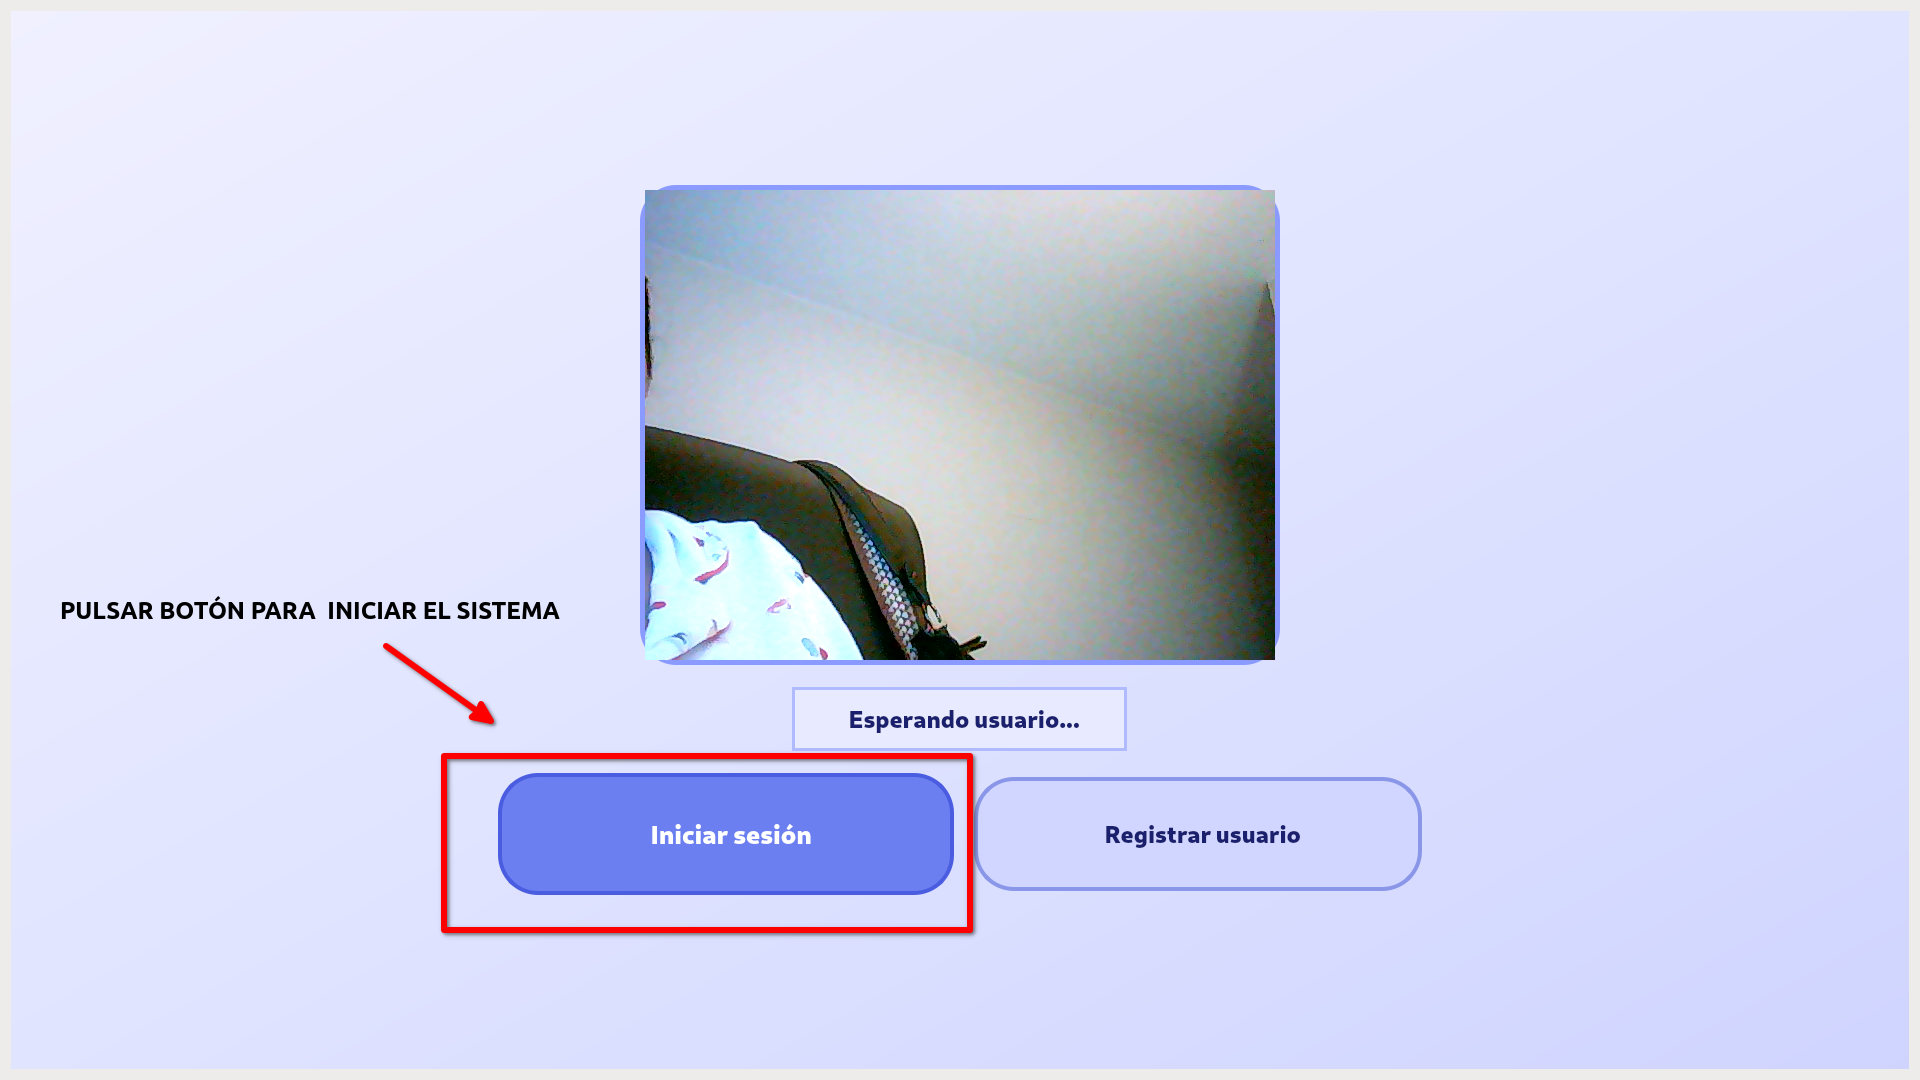
\includegraphics[width=0.9\textwidth]{figs/inicio}
    \caption{Pantallas de inicio de sesión}
    \label{fig:inicio}
\end{figure}


Una vez completada la autenticación, el sistema identifica al usuario y muestra su nombre en la pantalla.

\vspace{0.2cm}

\begin{figure}[H]
    \centering
    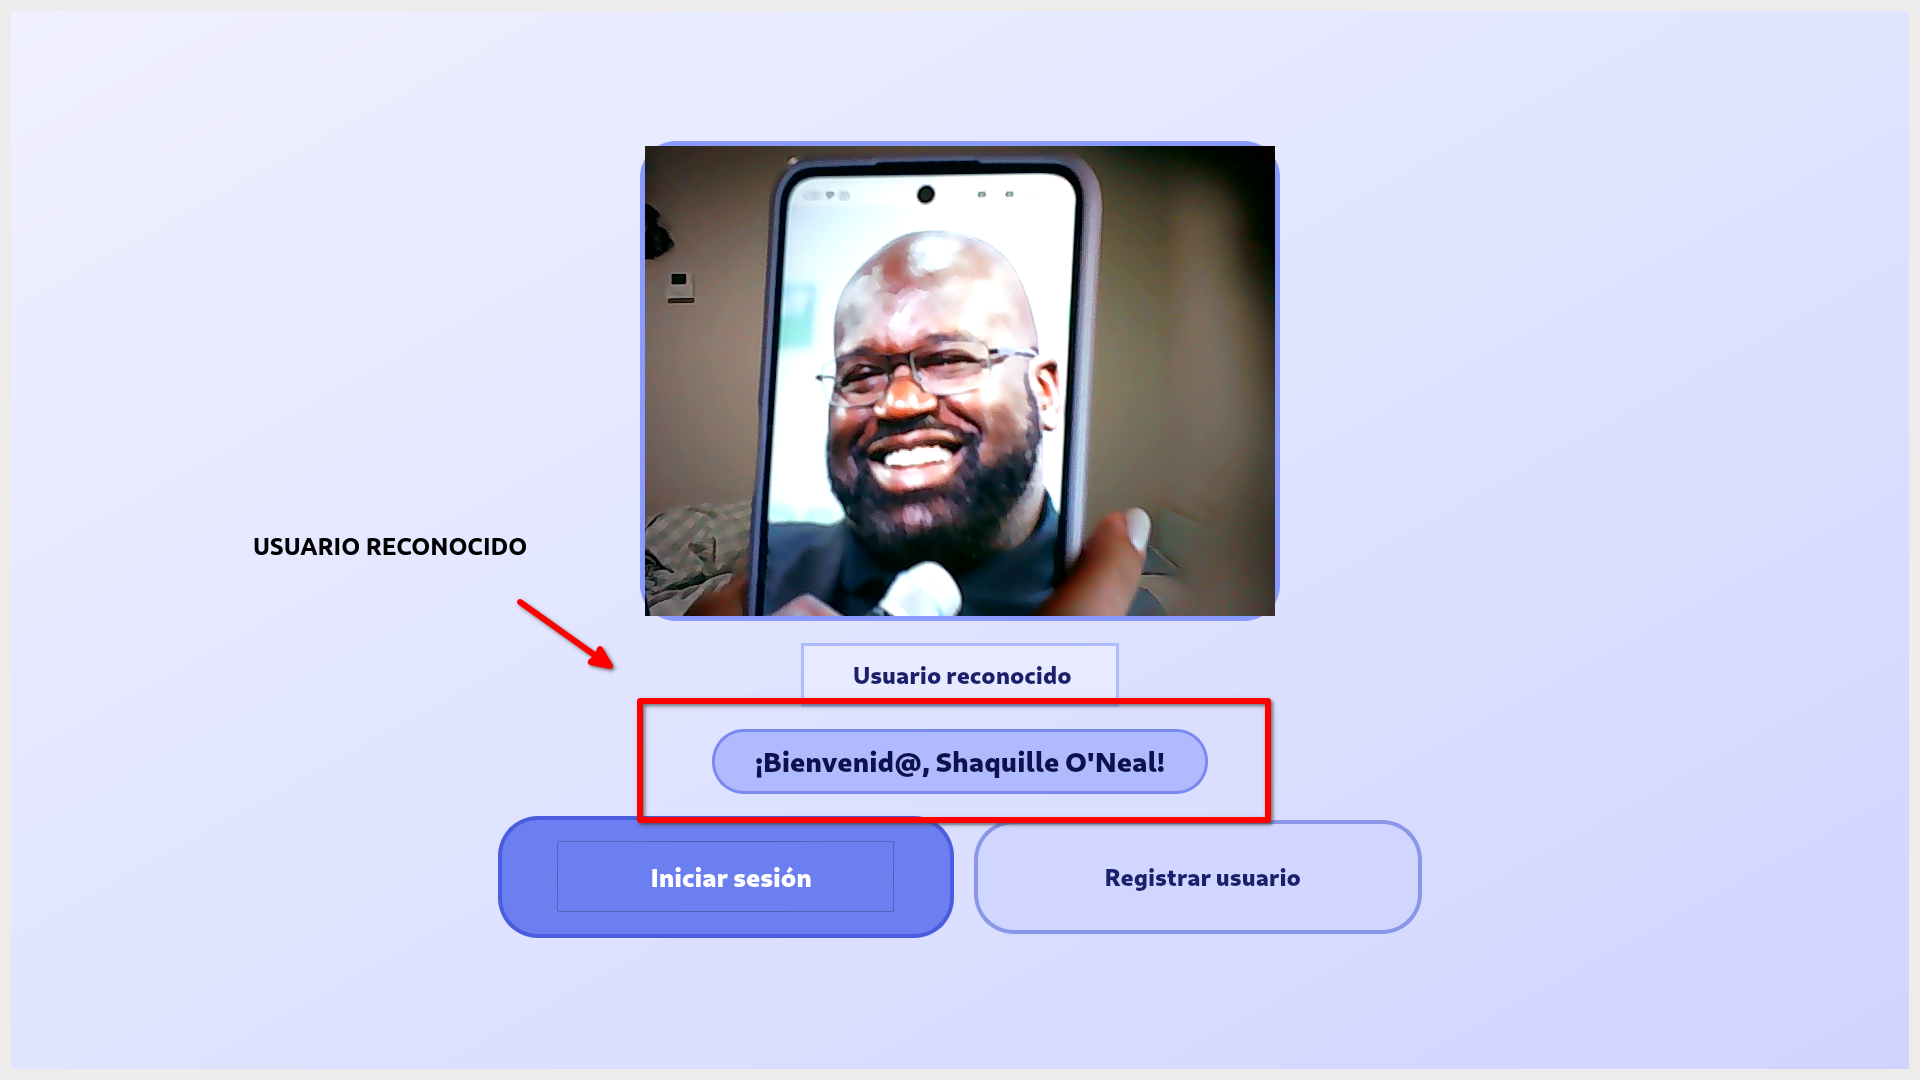
\includegraphics[width=0.9\textwidth]{figs/reconocido}
    \caption{Usuario identificado}
    \label{fig:reconocido}
\end{figure}


\vspace{0.2cm}

Si el usuario no se encuentra registrado, es posible registrar un nuevo usuario siguiendo un sencillo proceso de registro:


\vspace{0.2cm}


\textbf{Paso 1:} Introducir el nombre del nuevo usuario.\\

\vspace{0.2cm}

\begin{figure}[H]
    \centering
    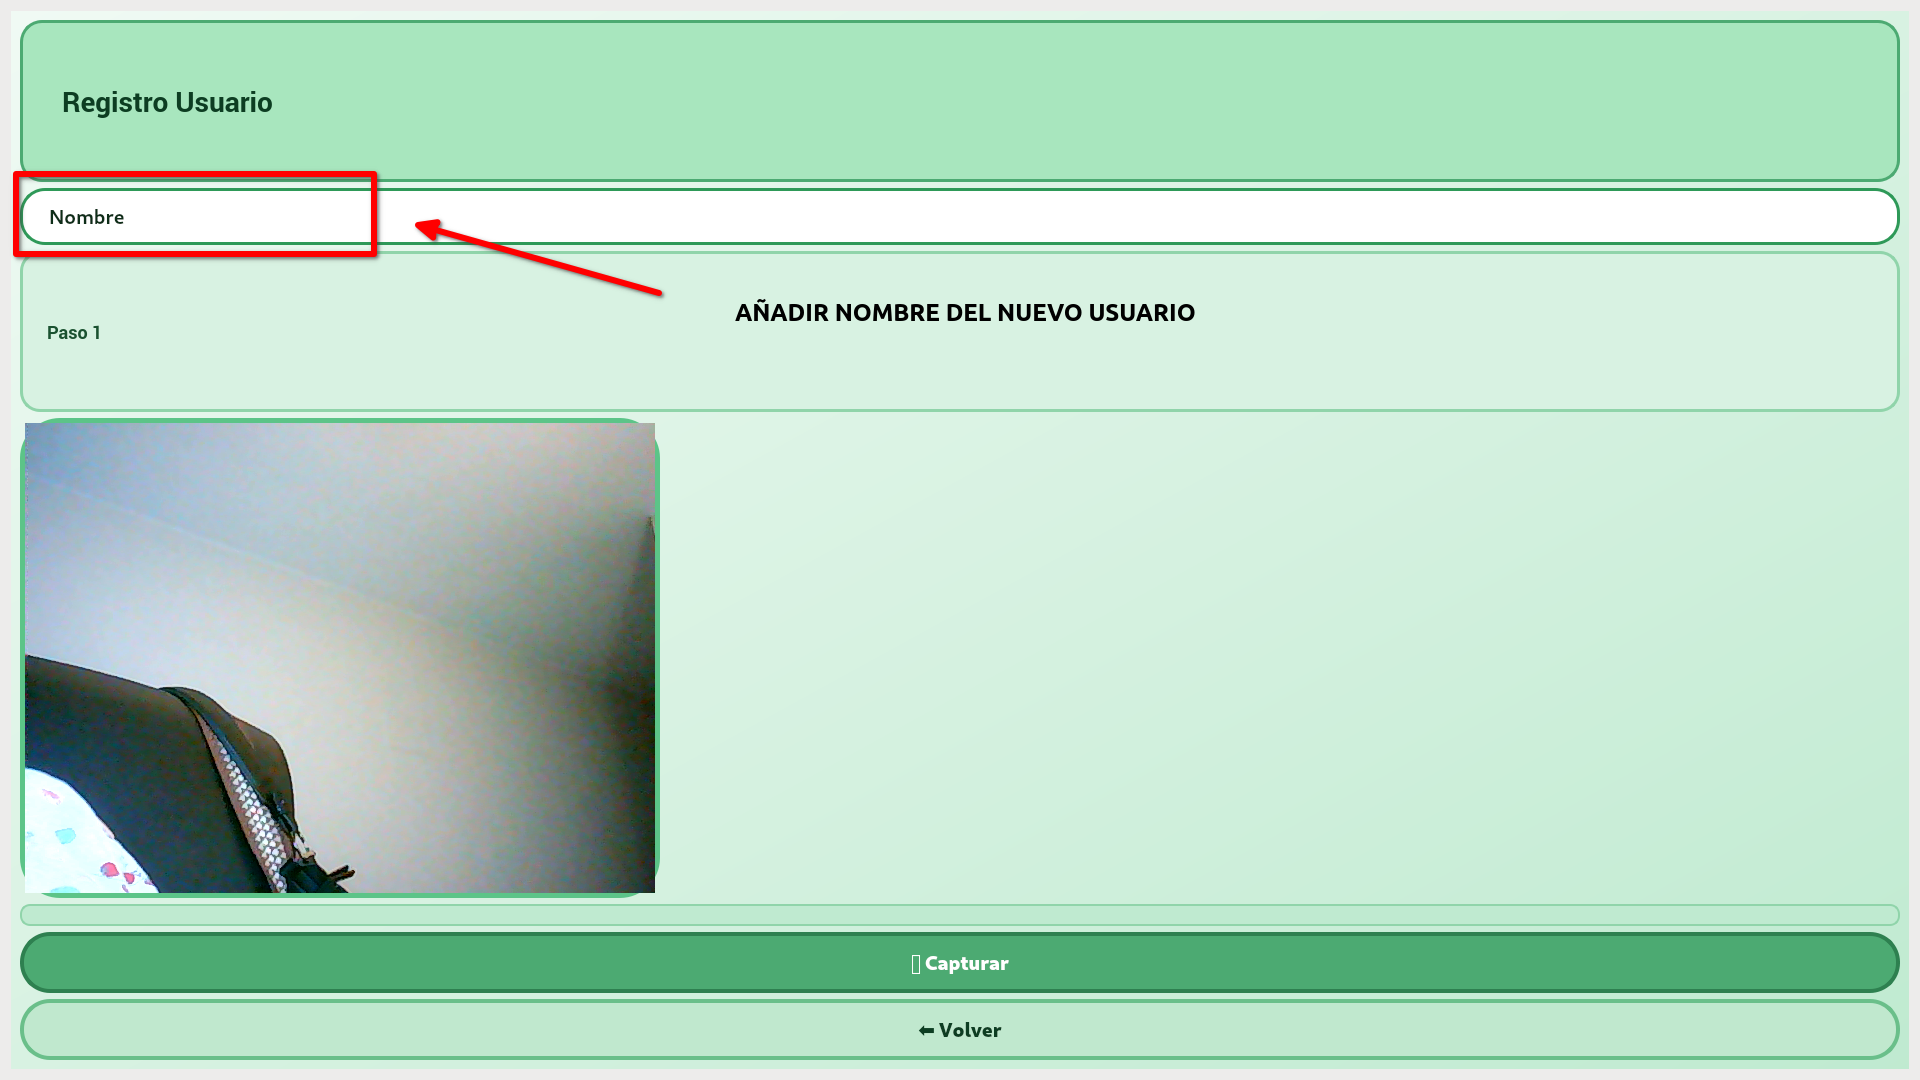
\includegraphics[width=0.9\textwidth]{figs/registro}
    \caption{Registro de nuevo usuario}
    \label{fig:registro}
\end{figure}


\textbf{Paso 2:} Capturar tres imágenes del rostro desde diferentes posiciones.\\

\vspace{0.2cm}

\begin{figure}[H]
    \centering
    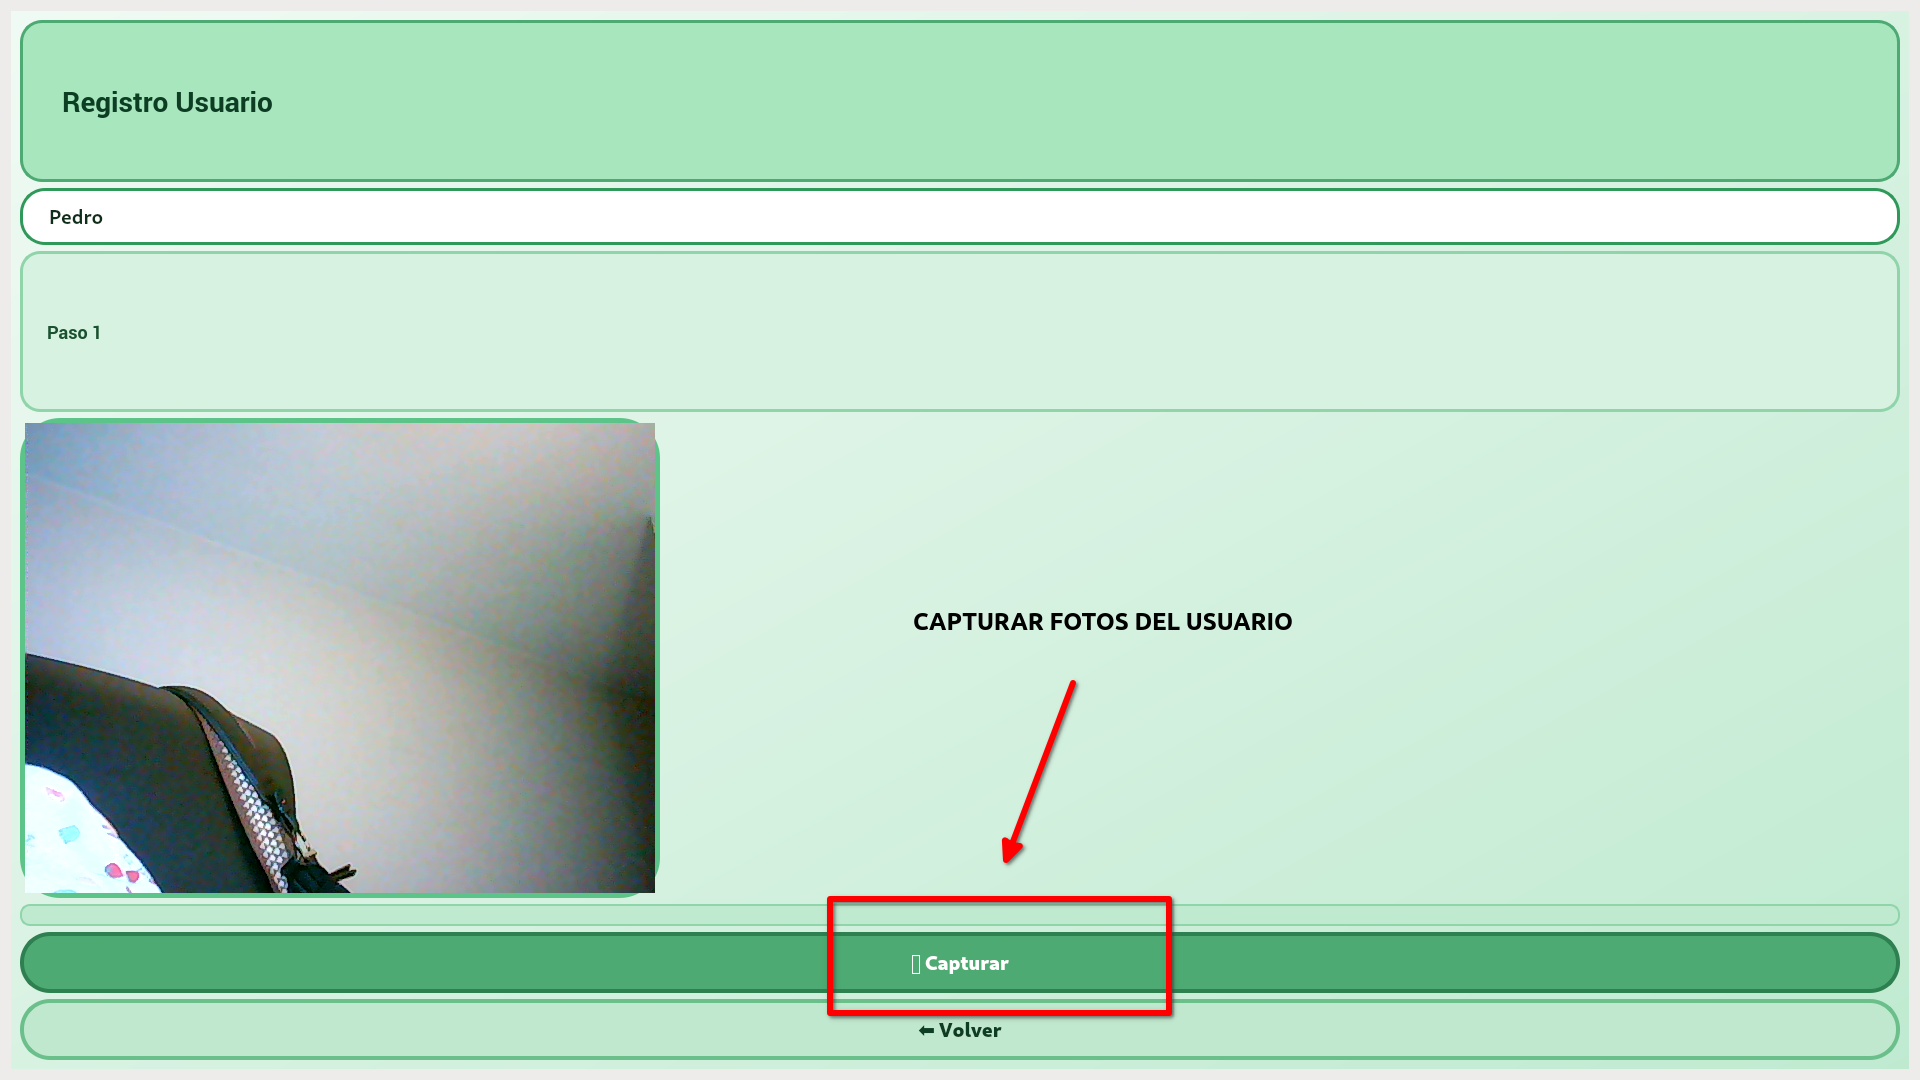
\includegraphics[width=0.9\textwidth]{figs/capturar}
    \caption{Captura de foto de usuario}
    \label{fig:capturar}
\end{figure}


Una vez completado el registro, el usuario puede autenticarse y acceder a las funcionalidades del robot.

\begin{figure}[H]
    \centering
    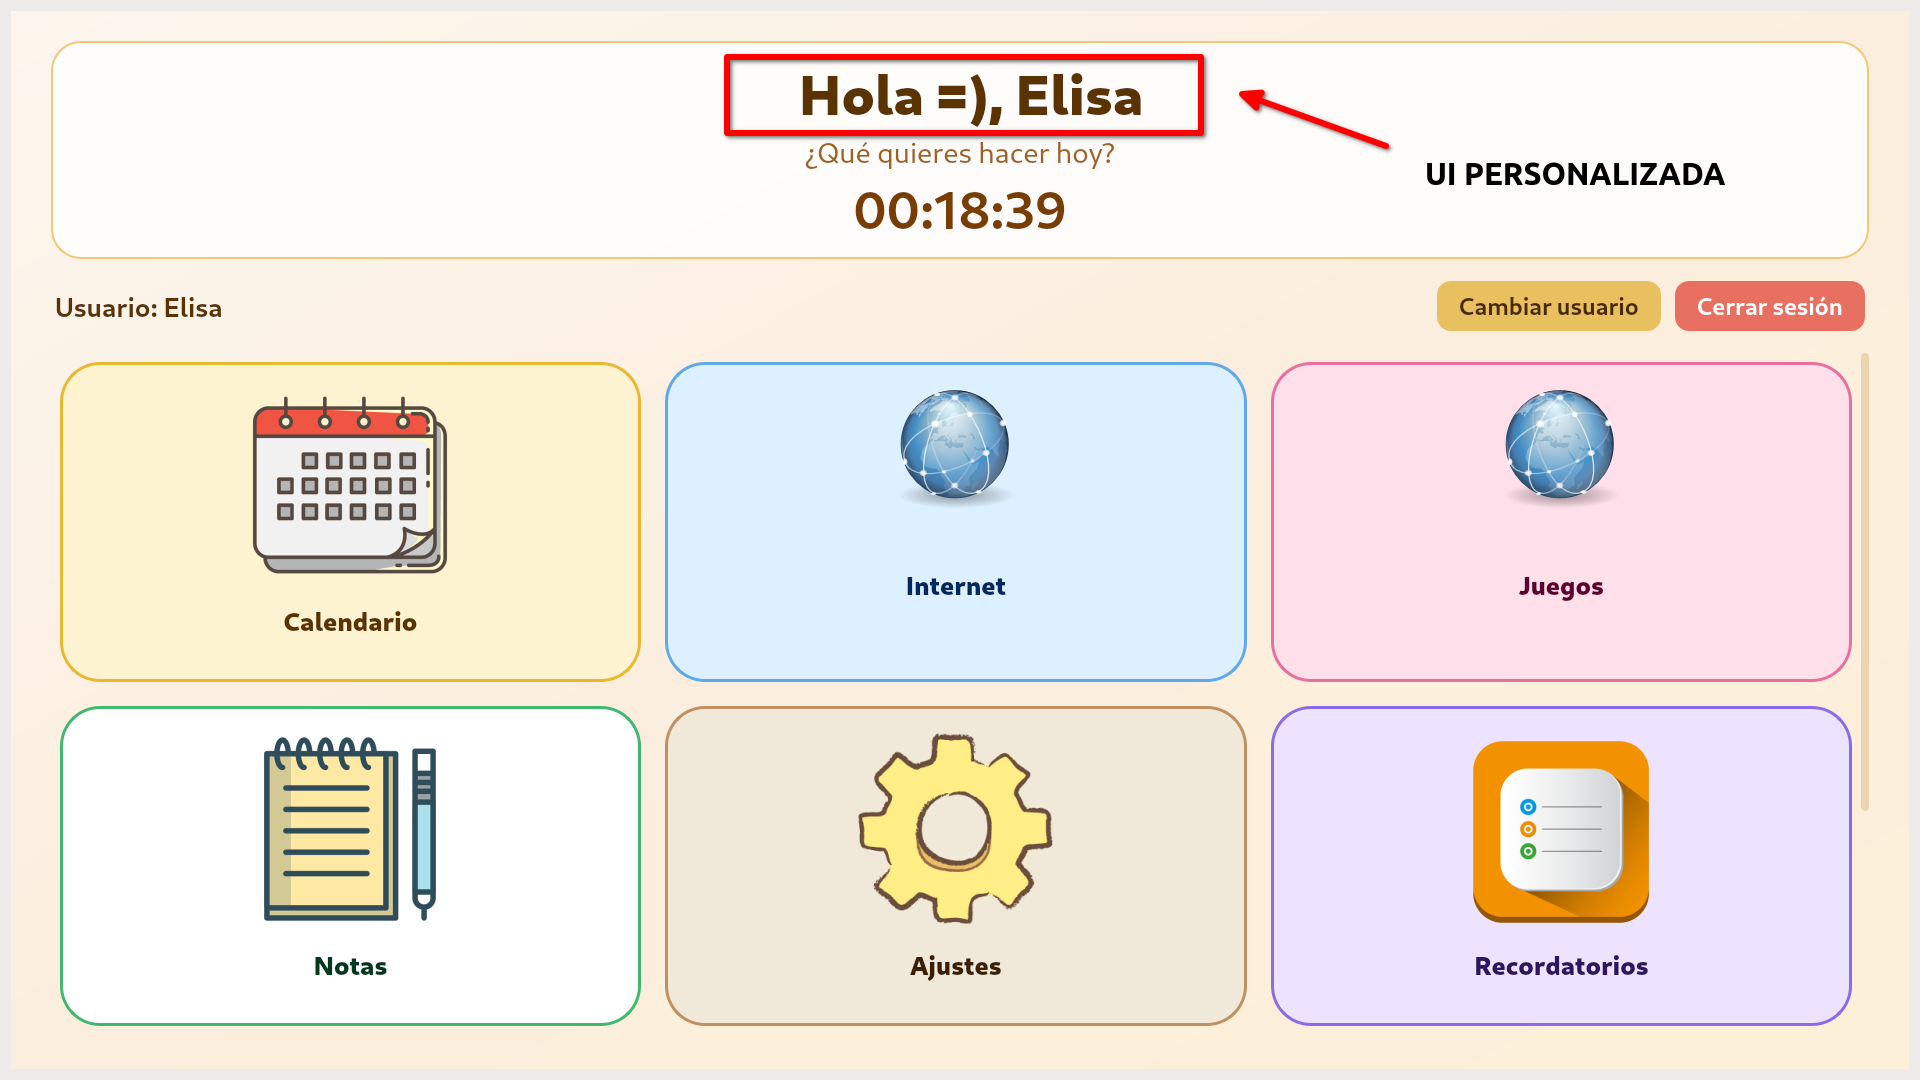
\includegraphics[width=0.9\textwidth]{figs/ui-nombre}
    \caption{UI del usuario}
    \label{fig:ui-nombre}
\end{figure}


\section{Interacción por voz}

Tras iniciar la interfaz gráfica, el robot activa el sistema de escucha. Permanecerá en estado de escucha pasiva, esperando una de las palabras de activación para iniciar la interacción.

Mientras permanece en estado de espera, la pantalla LCD muestra el estado actual del robot.

\vspace{0.2cm}

\begin{figure}[H]
    \centering
    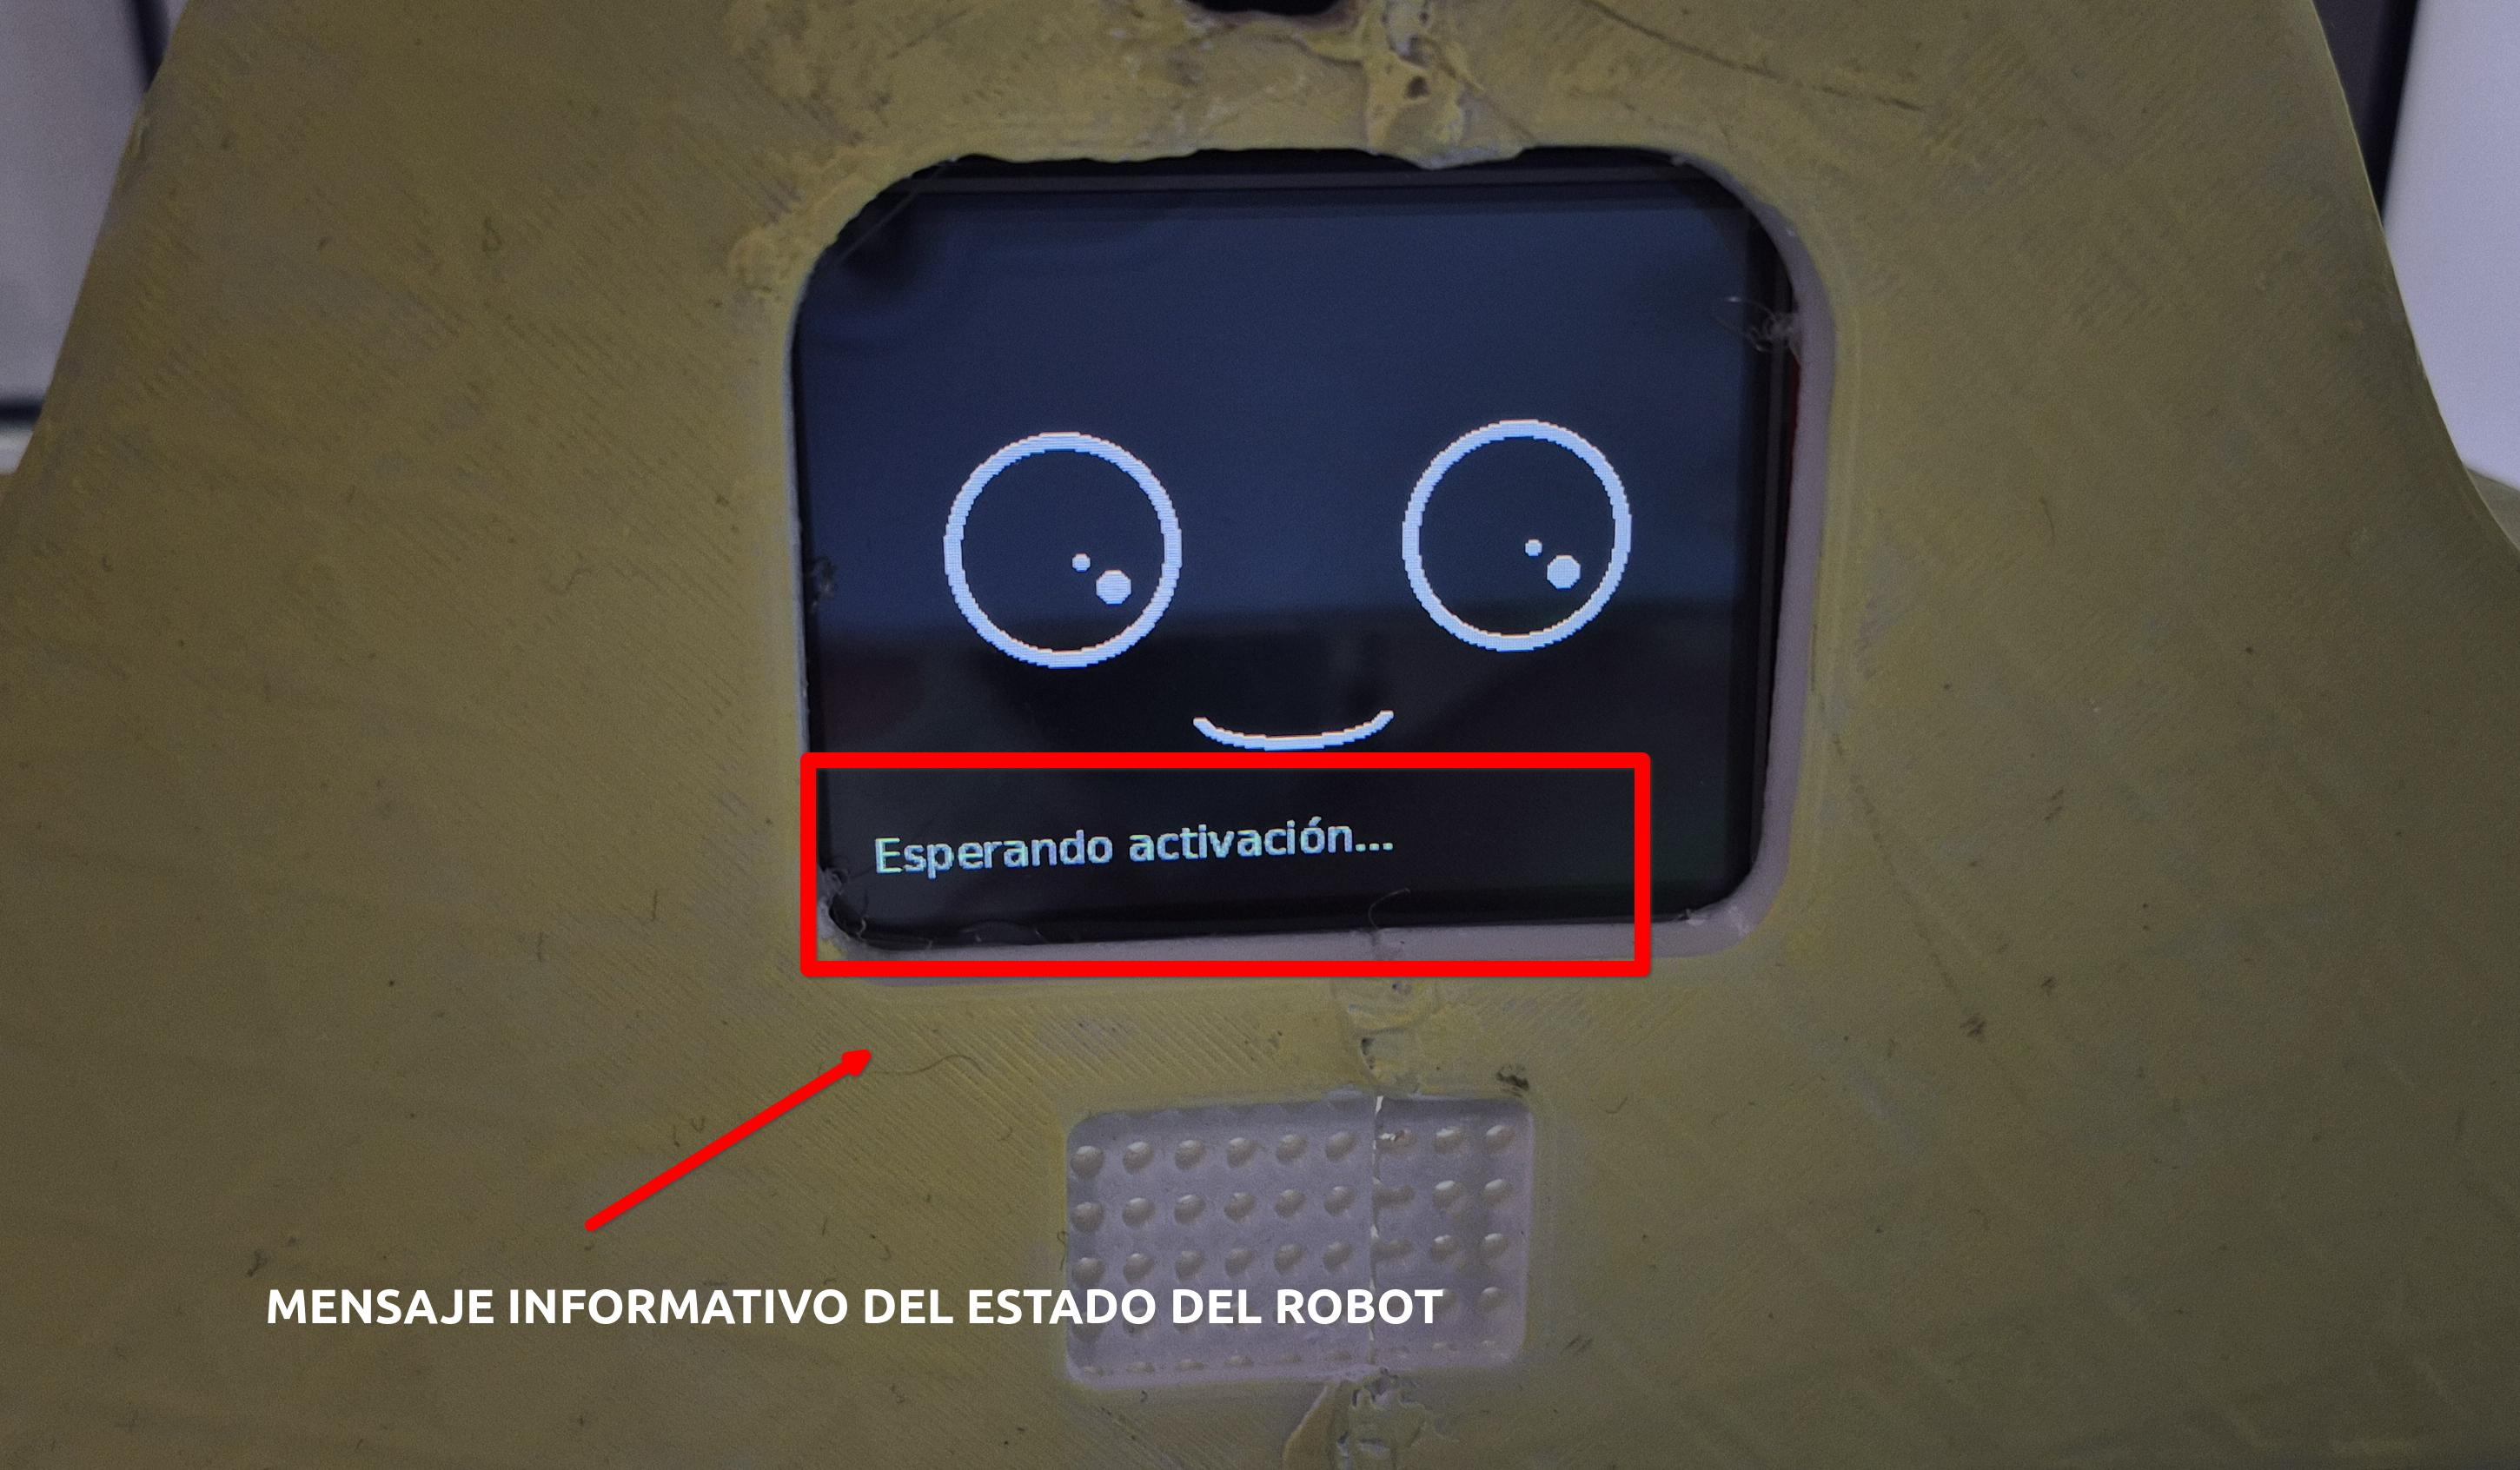
\includegraphics[width=0.9\textwidth]{figs/inf}
    \caption{Mensaje estado activación}
    \label{fig:inf}
\end{figure}


Las palabras de activación disponibles son \textit{«Oye»}, \textit{«Háblame»} y \textit{«Asistente»}.
Cuando el robot detecta cualquiera de estas palabras, inicia la escucha activa y actualiza el estado mostrado en la pantalla LCD para indicar que está escuchando al usuario.

\vspace{0.2cm}

\begin{figure}[H]
    \centering
    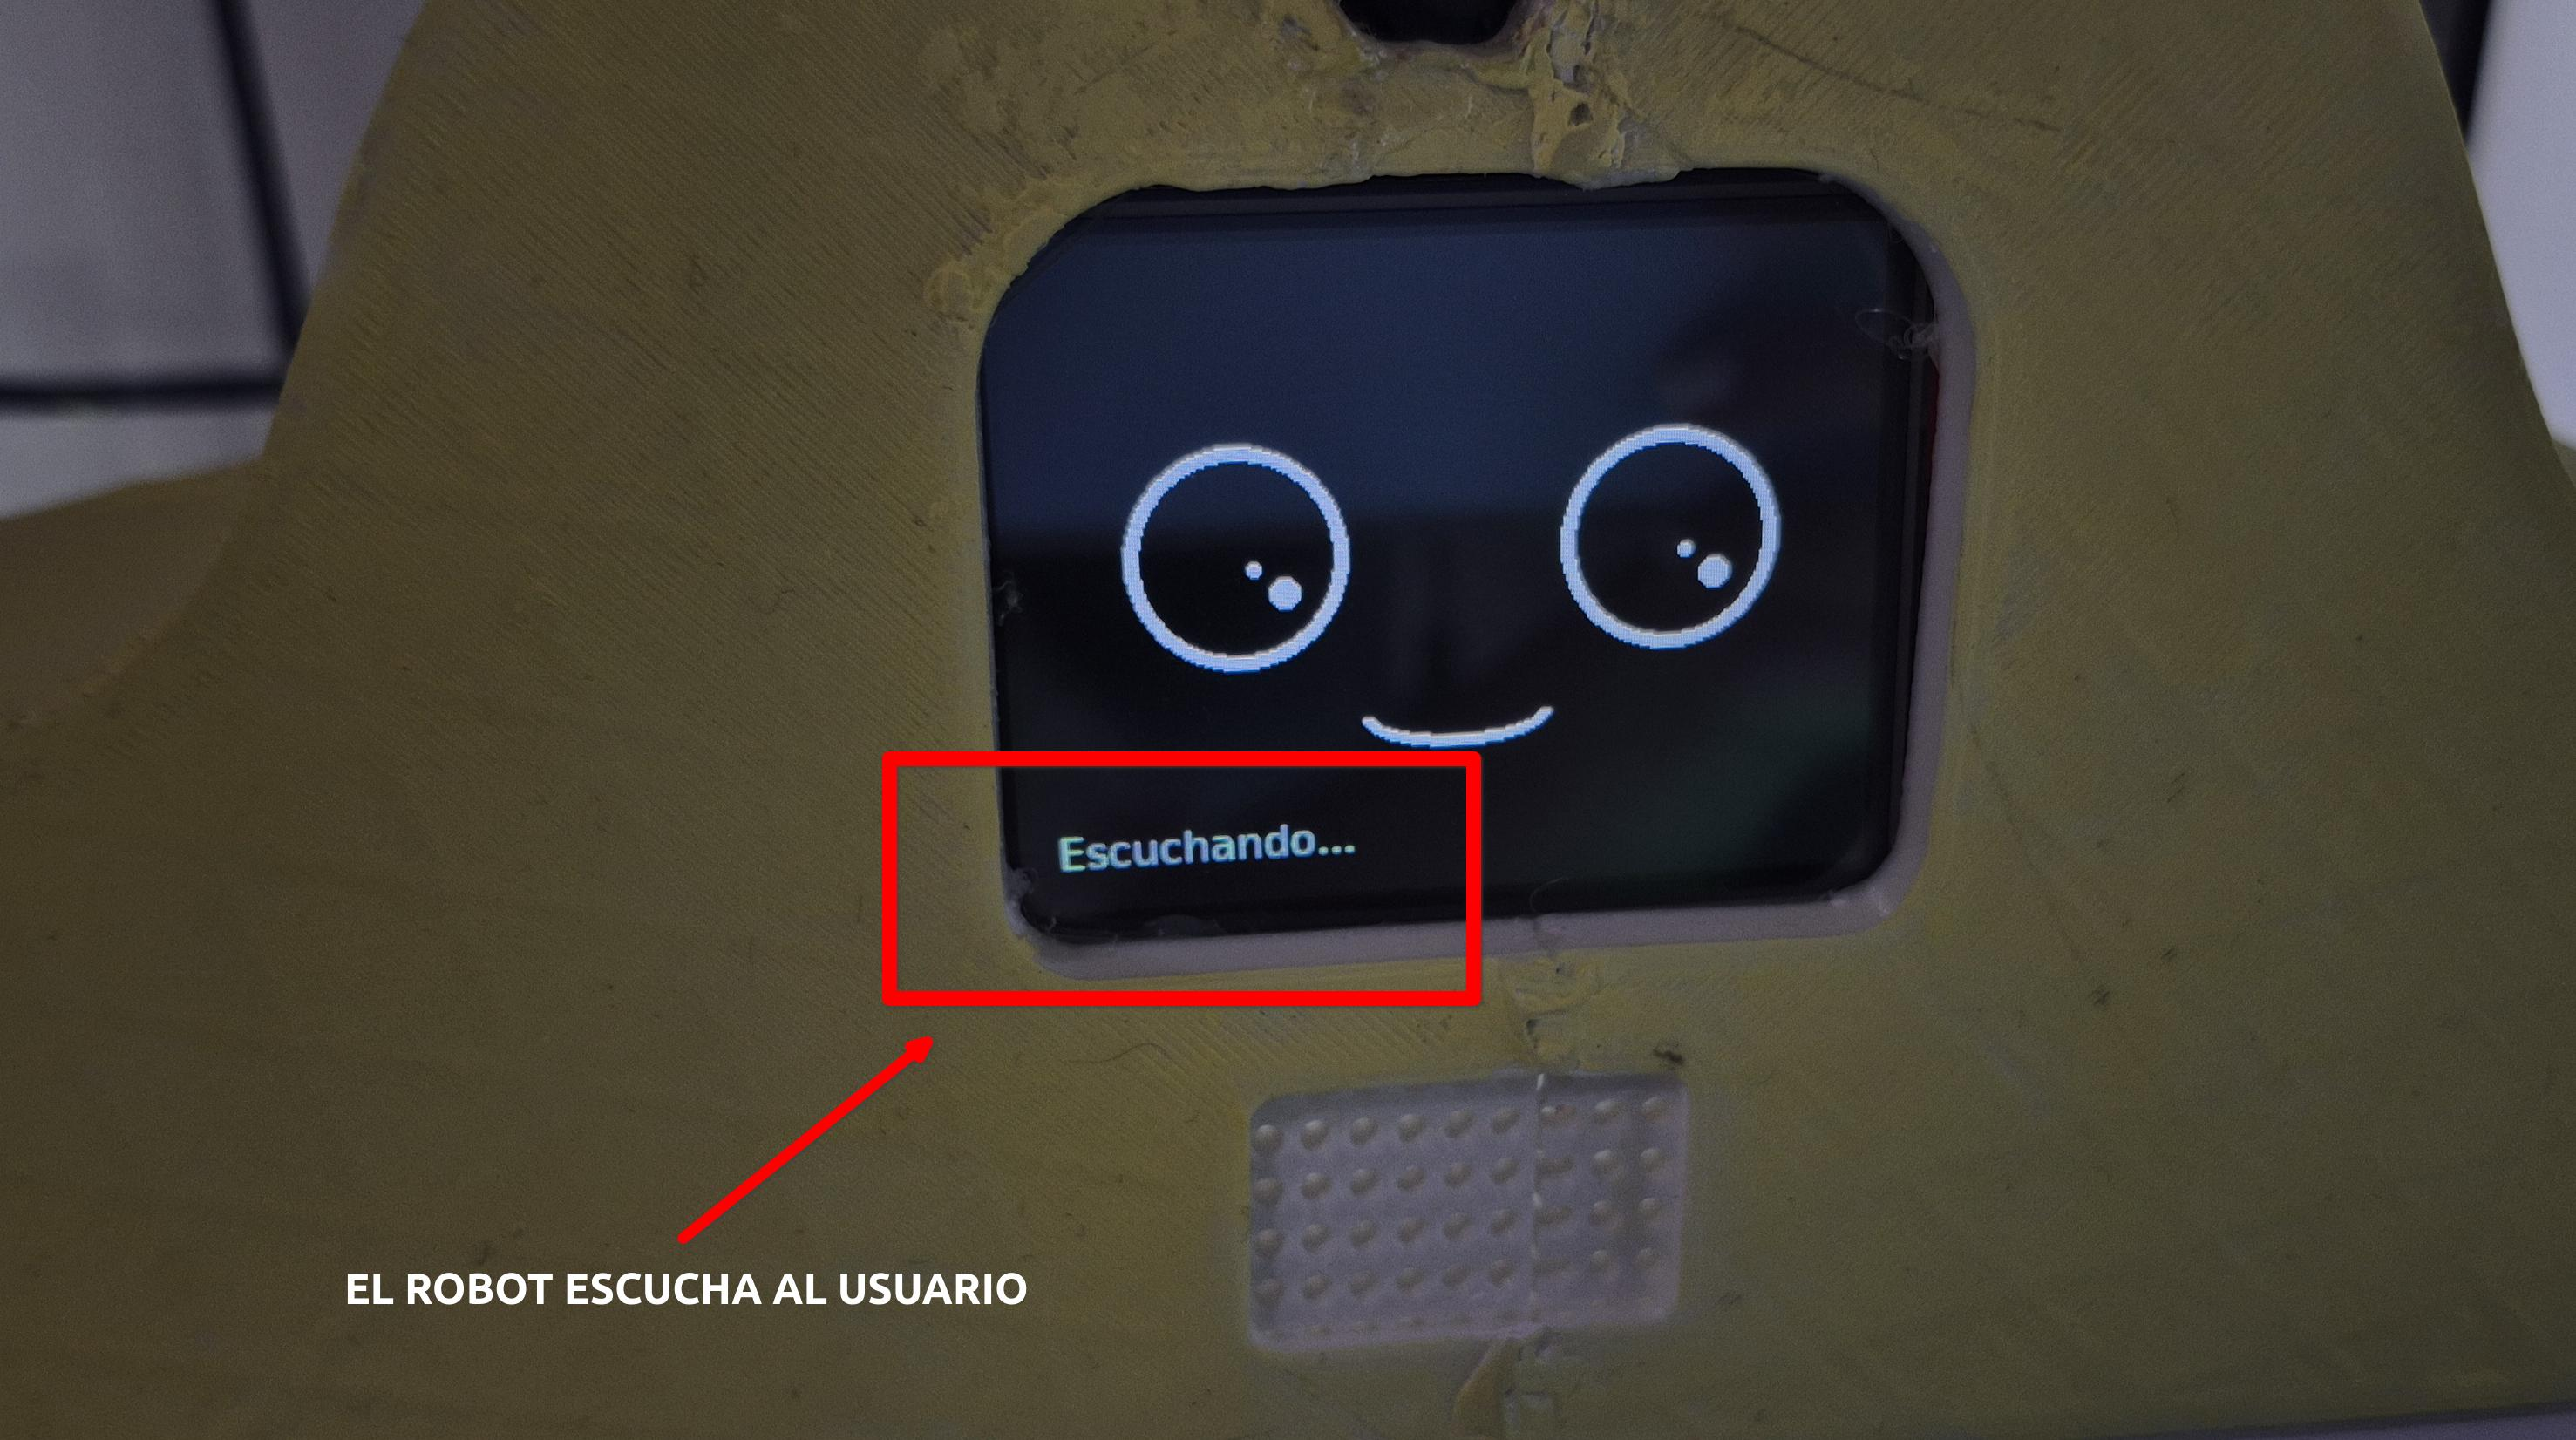
\includegraphics[width=0.9\textwidth]{figs/esc}
    \caption{Mensaje estado escuchando}
    \label{fig:esc}
\end{figure}


\section{Interacción con la interfaz del usuario}

La interfaz del robot incluye varias aplicaciones para el uso del usuario.

\vspace{0.2cm}


\subsection{Aplicación de calendario}

La aplicación de calendario permite añadir y eliminar eventos del usuario mediante una sencilla interfaz.

\vspace{0.2cm}

\begin{figure}[H]
    \centering
    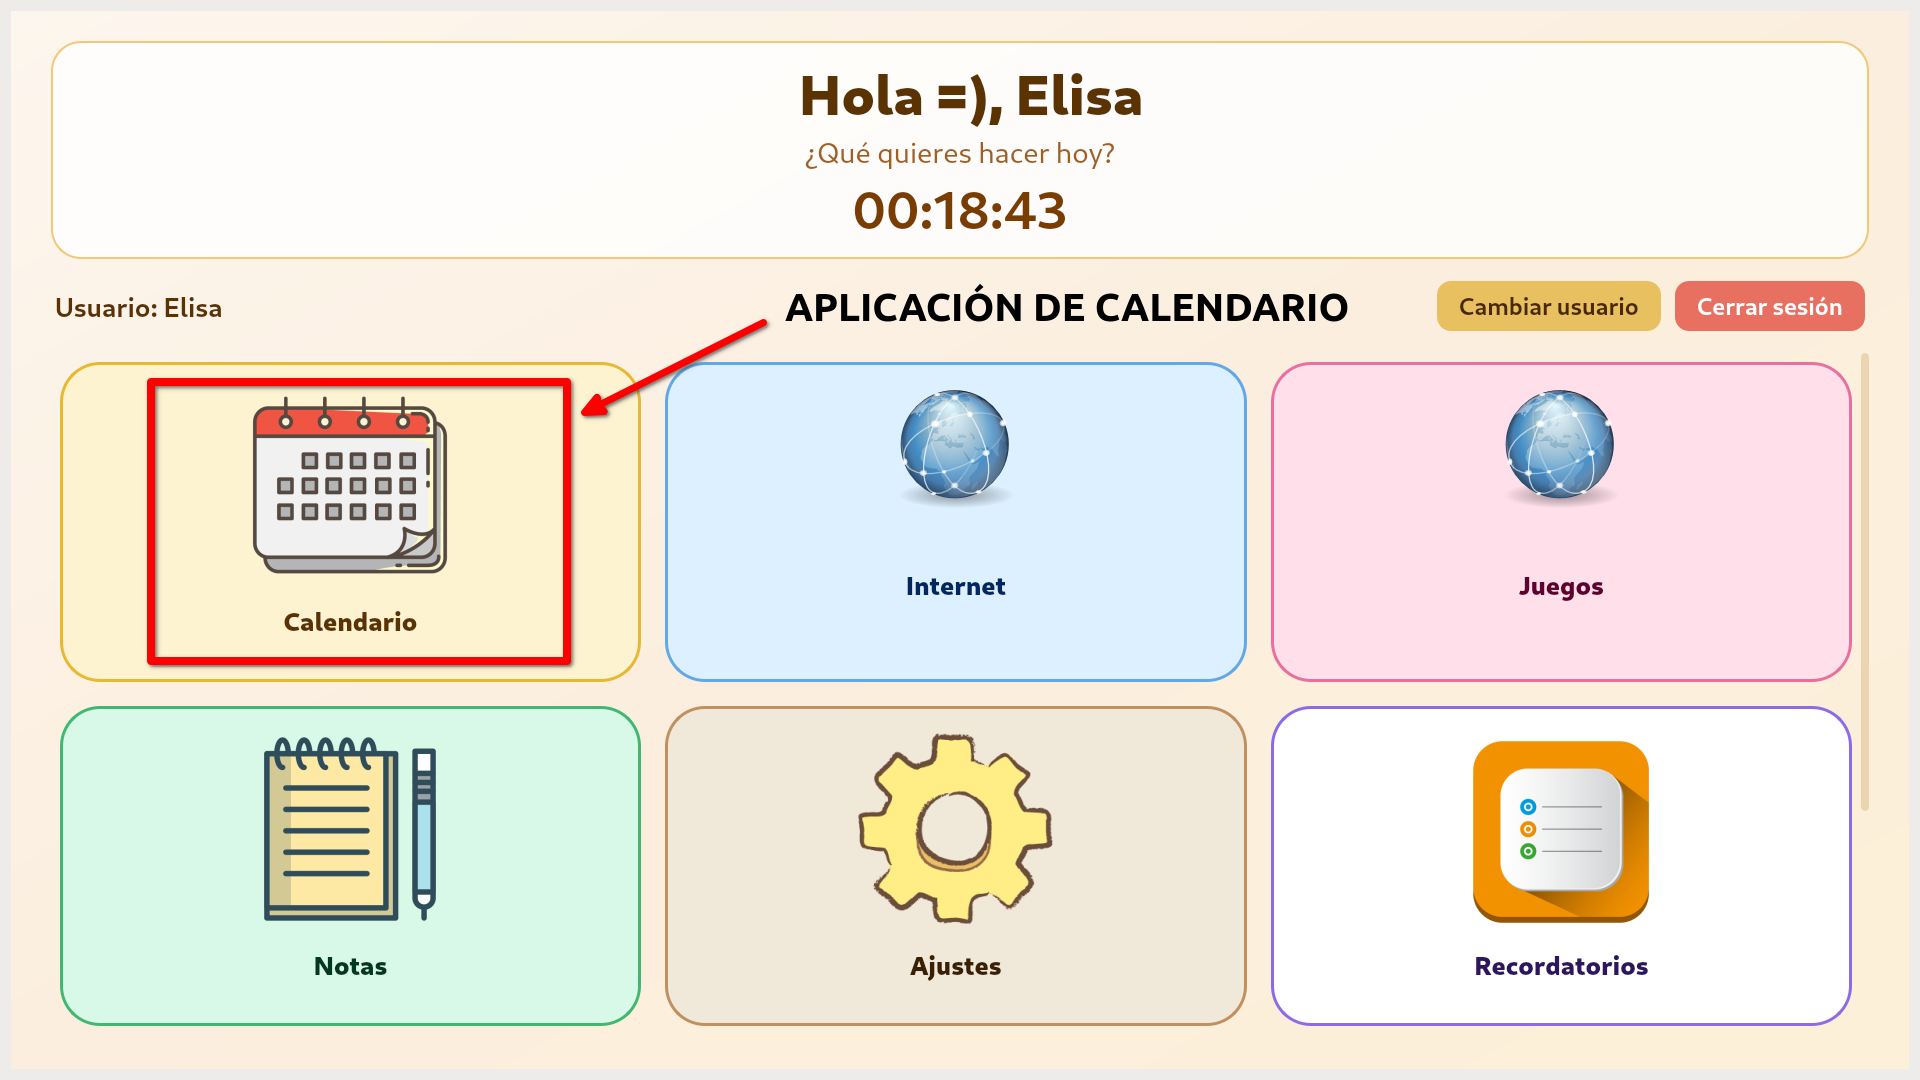
\includegraphics[width=0.9\textwidth]{figs/cal-app}
    \caption{Aplicación de calendario}
    \label{fig:cal-app}
\end{figure}


Para crear un nuevo evento, se deben seguir los siguientes pasos:

\textbf{Paso 1:} Seleccionar el día.\\

El usuario selecciona la fecha en la que desea crear el nuevo evento.

\begin{figure}[H]
    \centering
    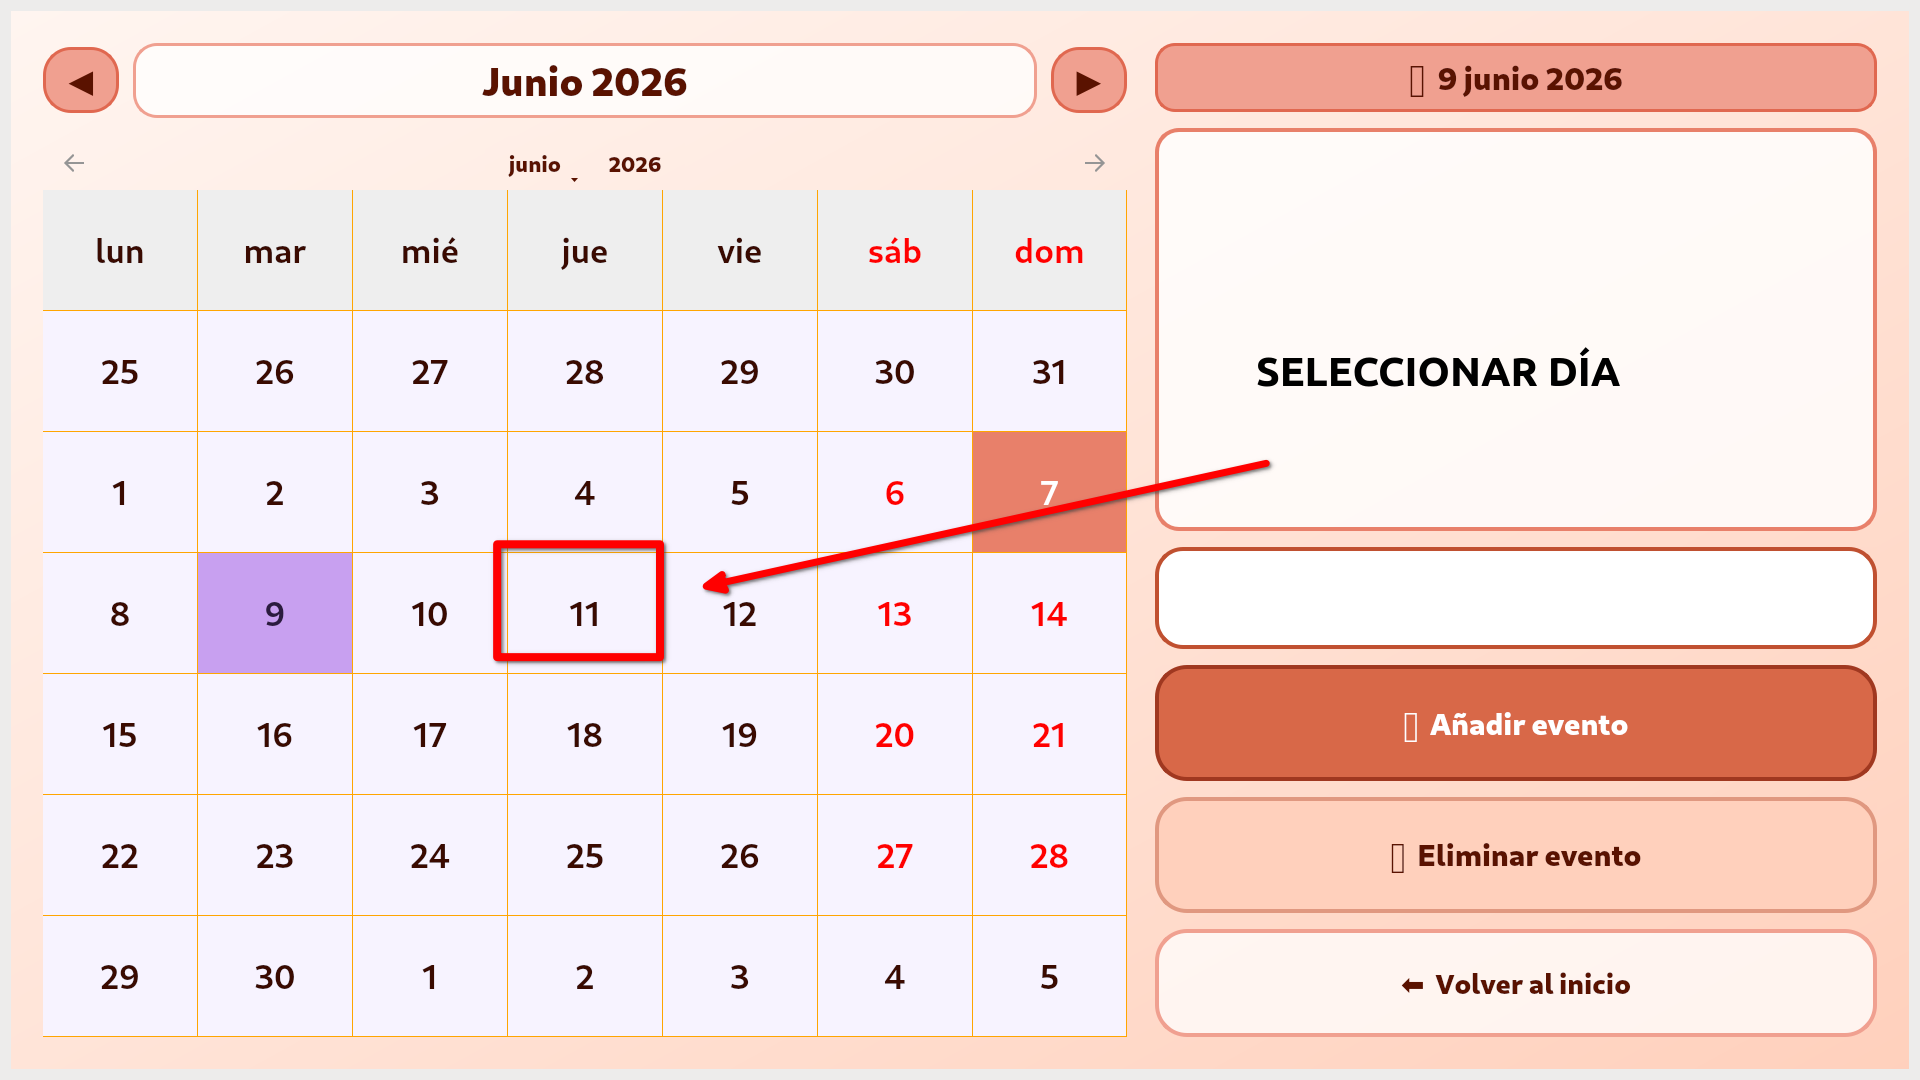
\includegraphics[width=0.9\textwidth]{figs/sel}
    \caption{Día seleccionado}
    \label{fig:sel}
\end{figure}


\textbf{Paso 2:} Introducir el nombre del evento.\\

Una vez seleccionada la fecha, se escribe el nombre del nuevo evento.

\vspace{0.2cm}


\begin{figure}[H]
    \centering
    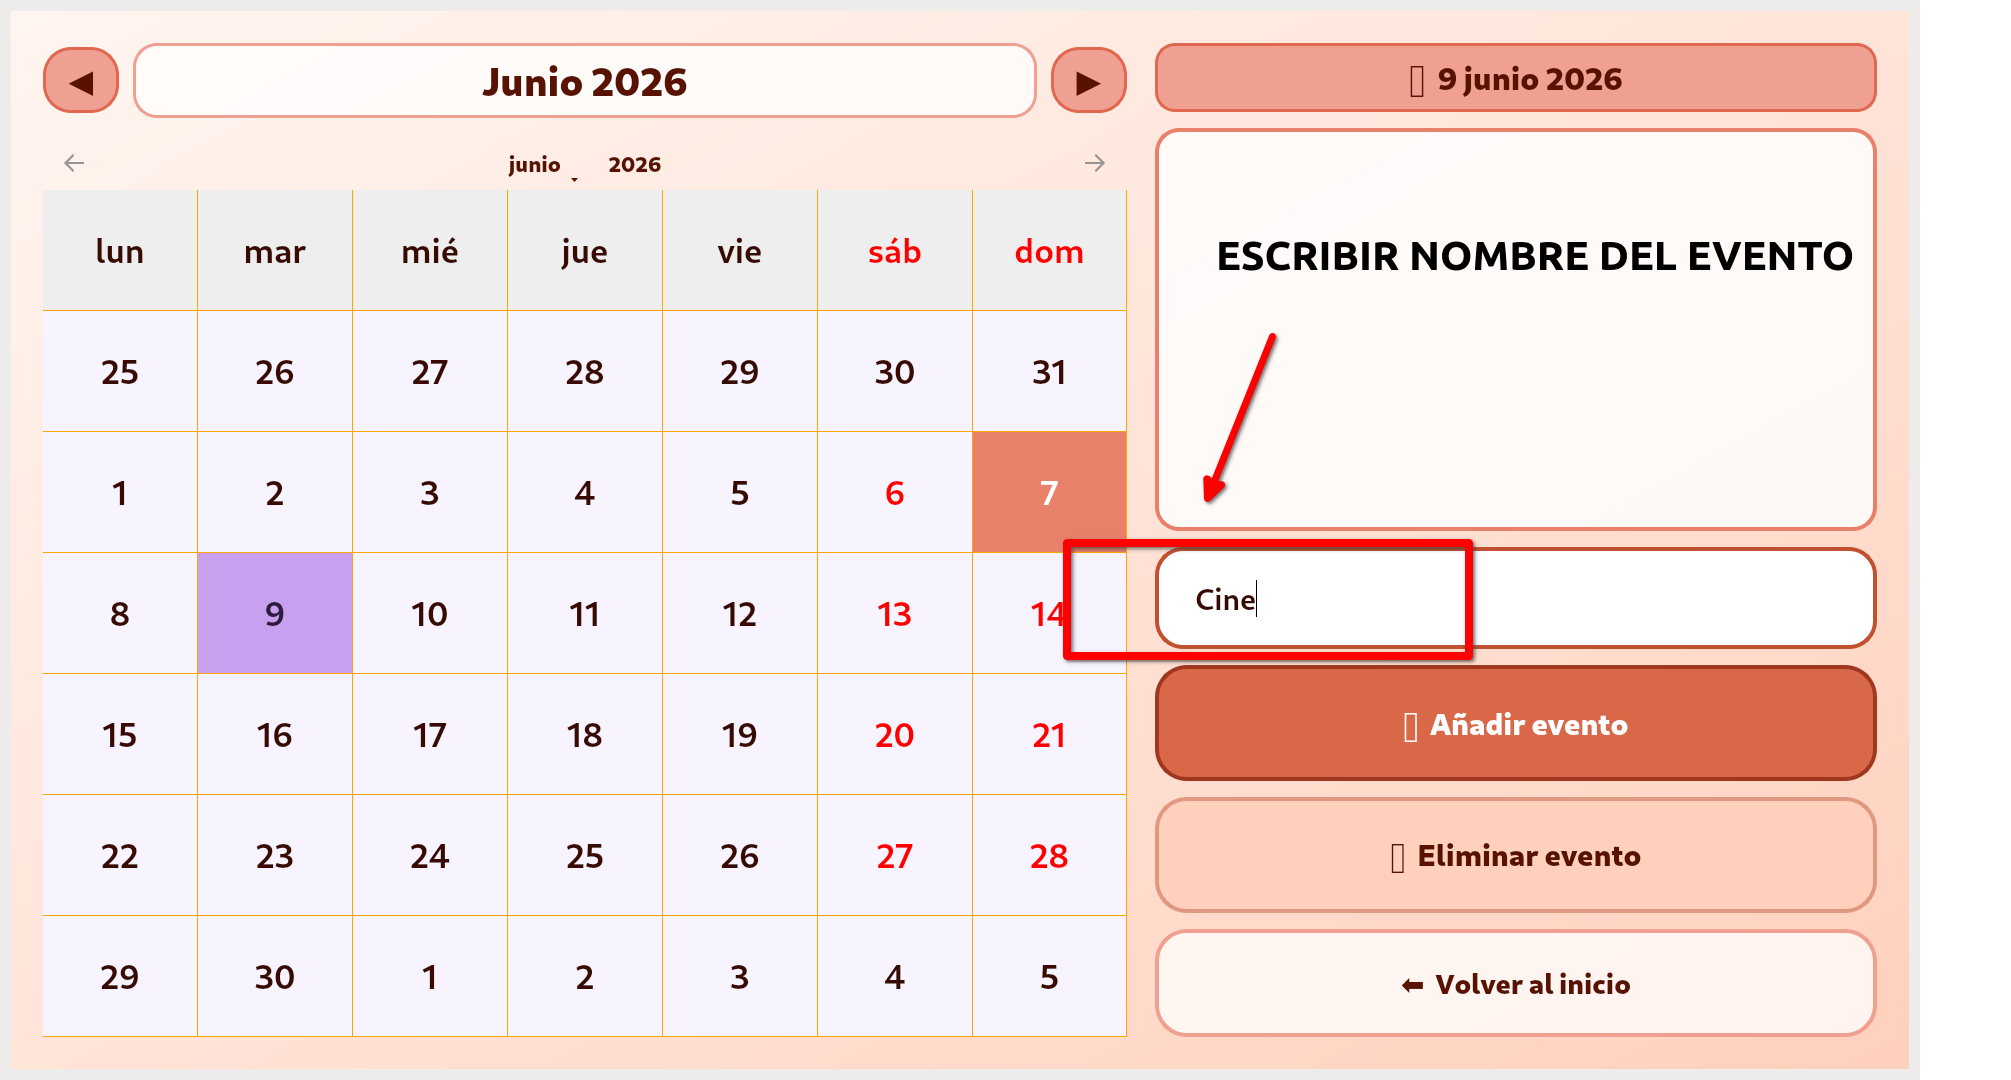
\includegraphics[width=0.9\textwidth]{figs/name}
    \caption{Escribir nombre del evento}
    \label{fig:name}
\end{figure}


\textbf{Paso 3:} Confirmar la creación del evento.\\

\vspace{0.2cm}

\begin{figure}[H]
    \centering
    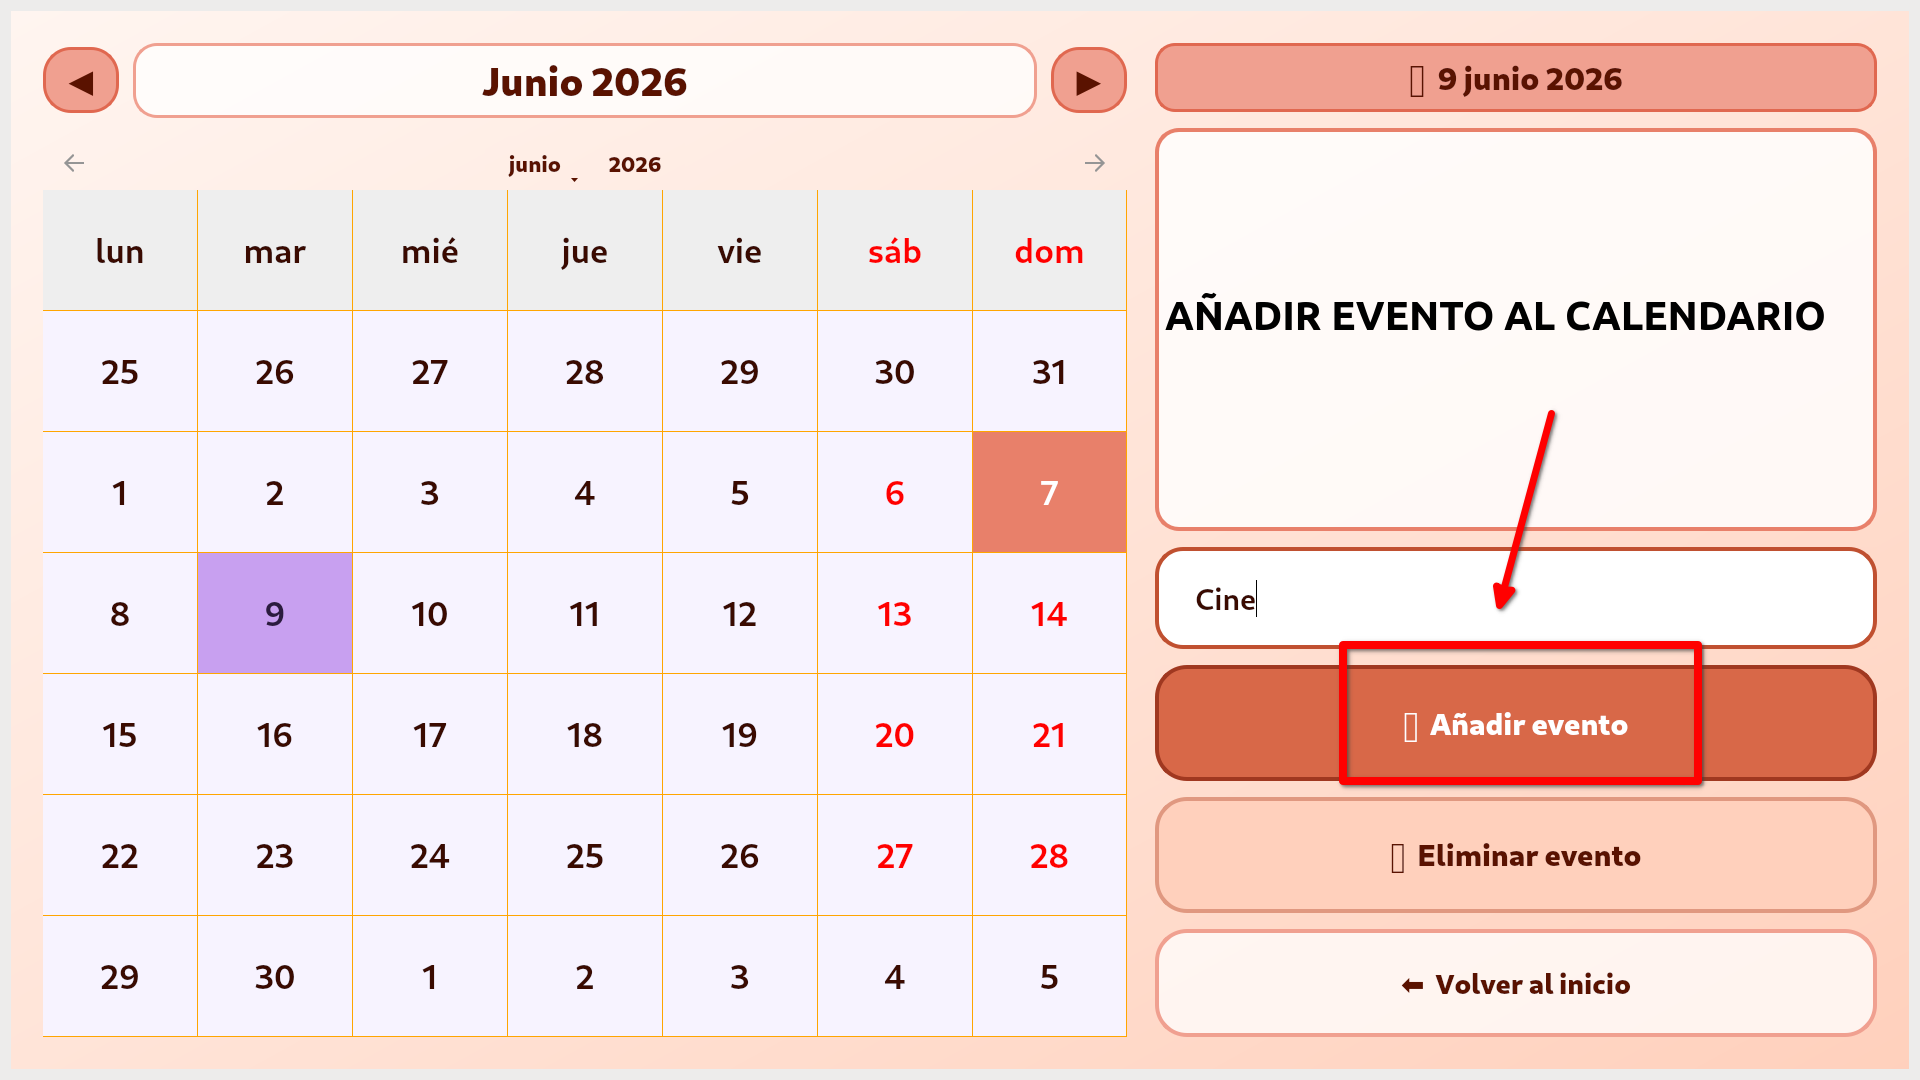
\includegraphics[width=0.9\textwidth]{figs/eve}
    \caption{Añadir el evento}
    \label{fig:eve}
\end{figure}


Tras confirmar la creación, el nuevo evento queda registrado y aparece en el calendario.

\begin{figure}[H]
    \centering
    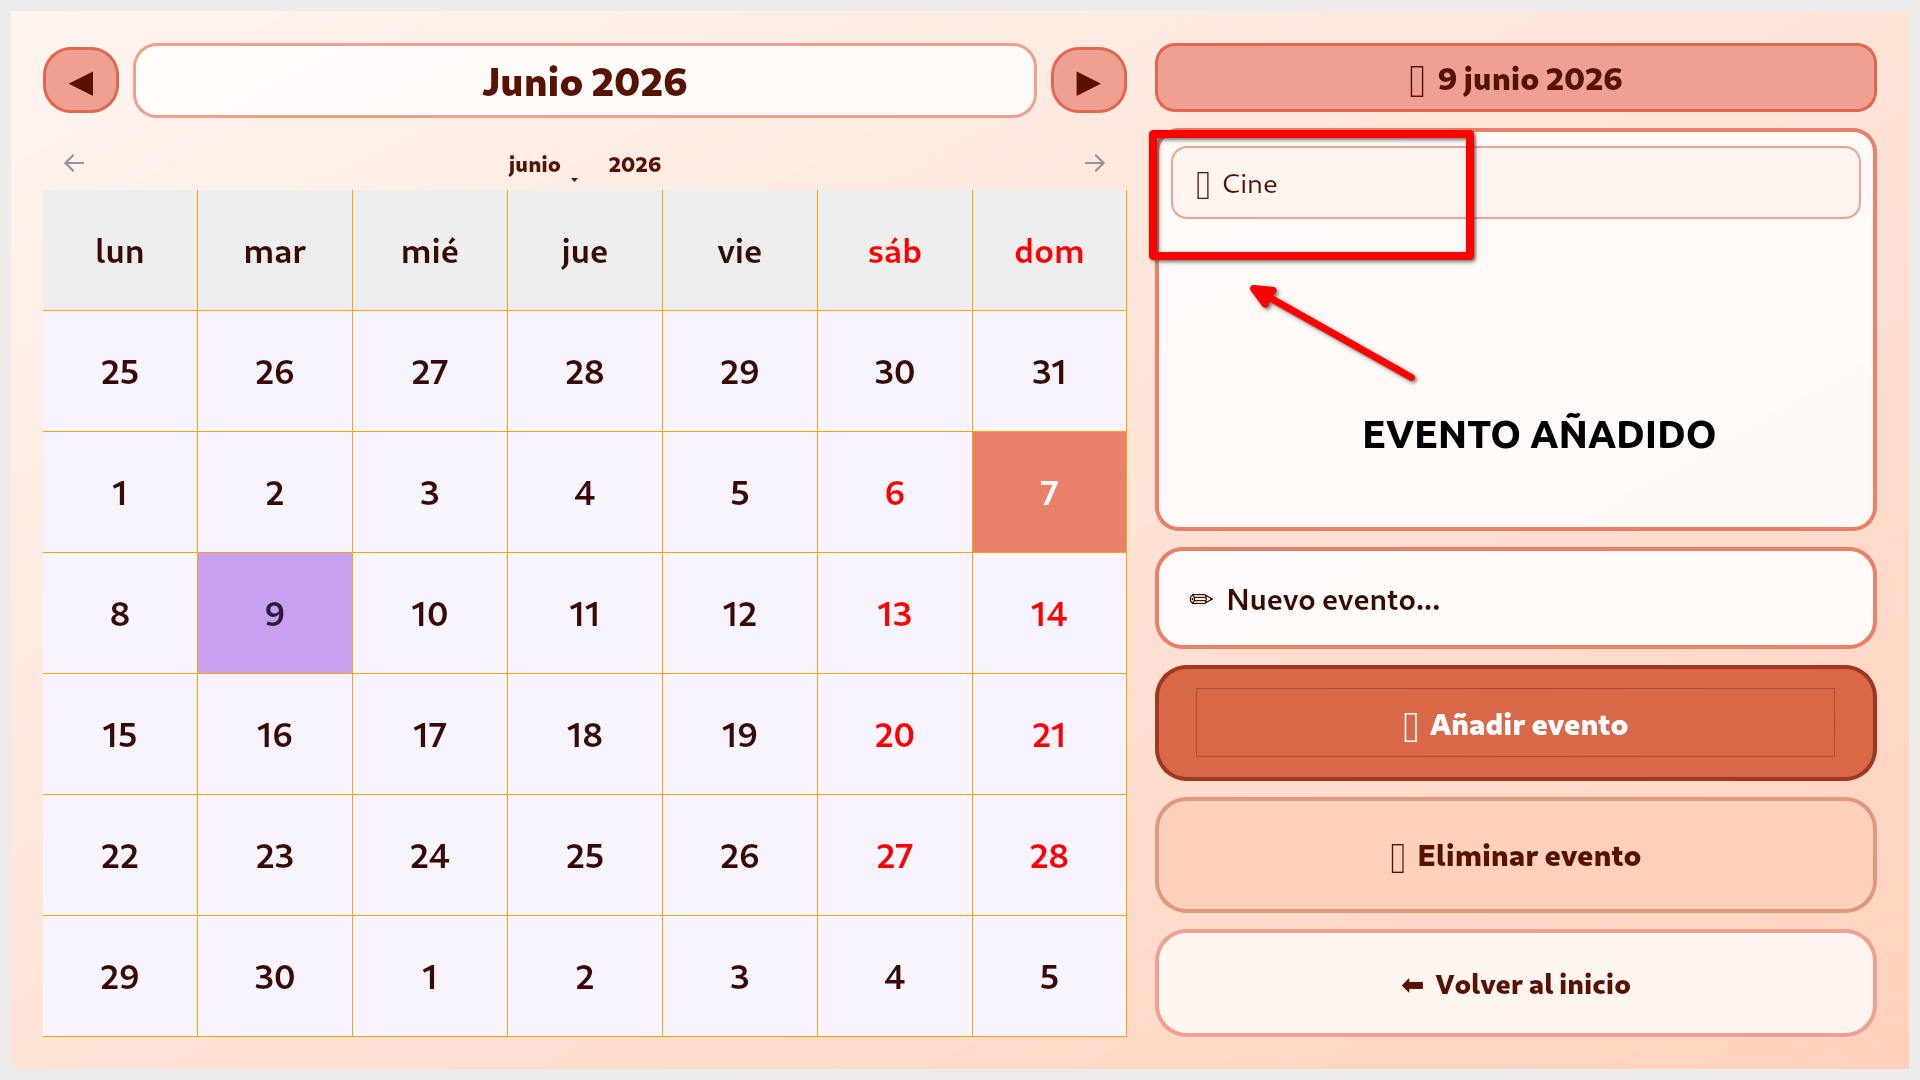
\includegraphics[width=0.9\textwidth]{figs/ev}
    \caption{Nuevo evento agregado}
    \label{fig:ev}
\end{figure}



La aplicación de calendario también permite eliminar eventos existentes.

\begin{figure}[H]
    \centering
    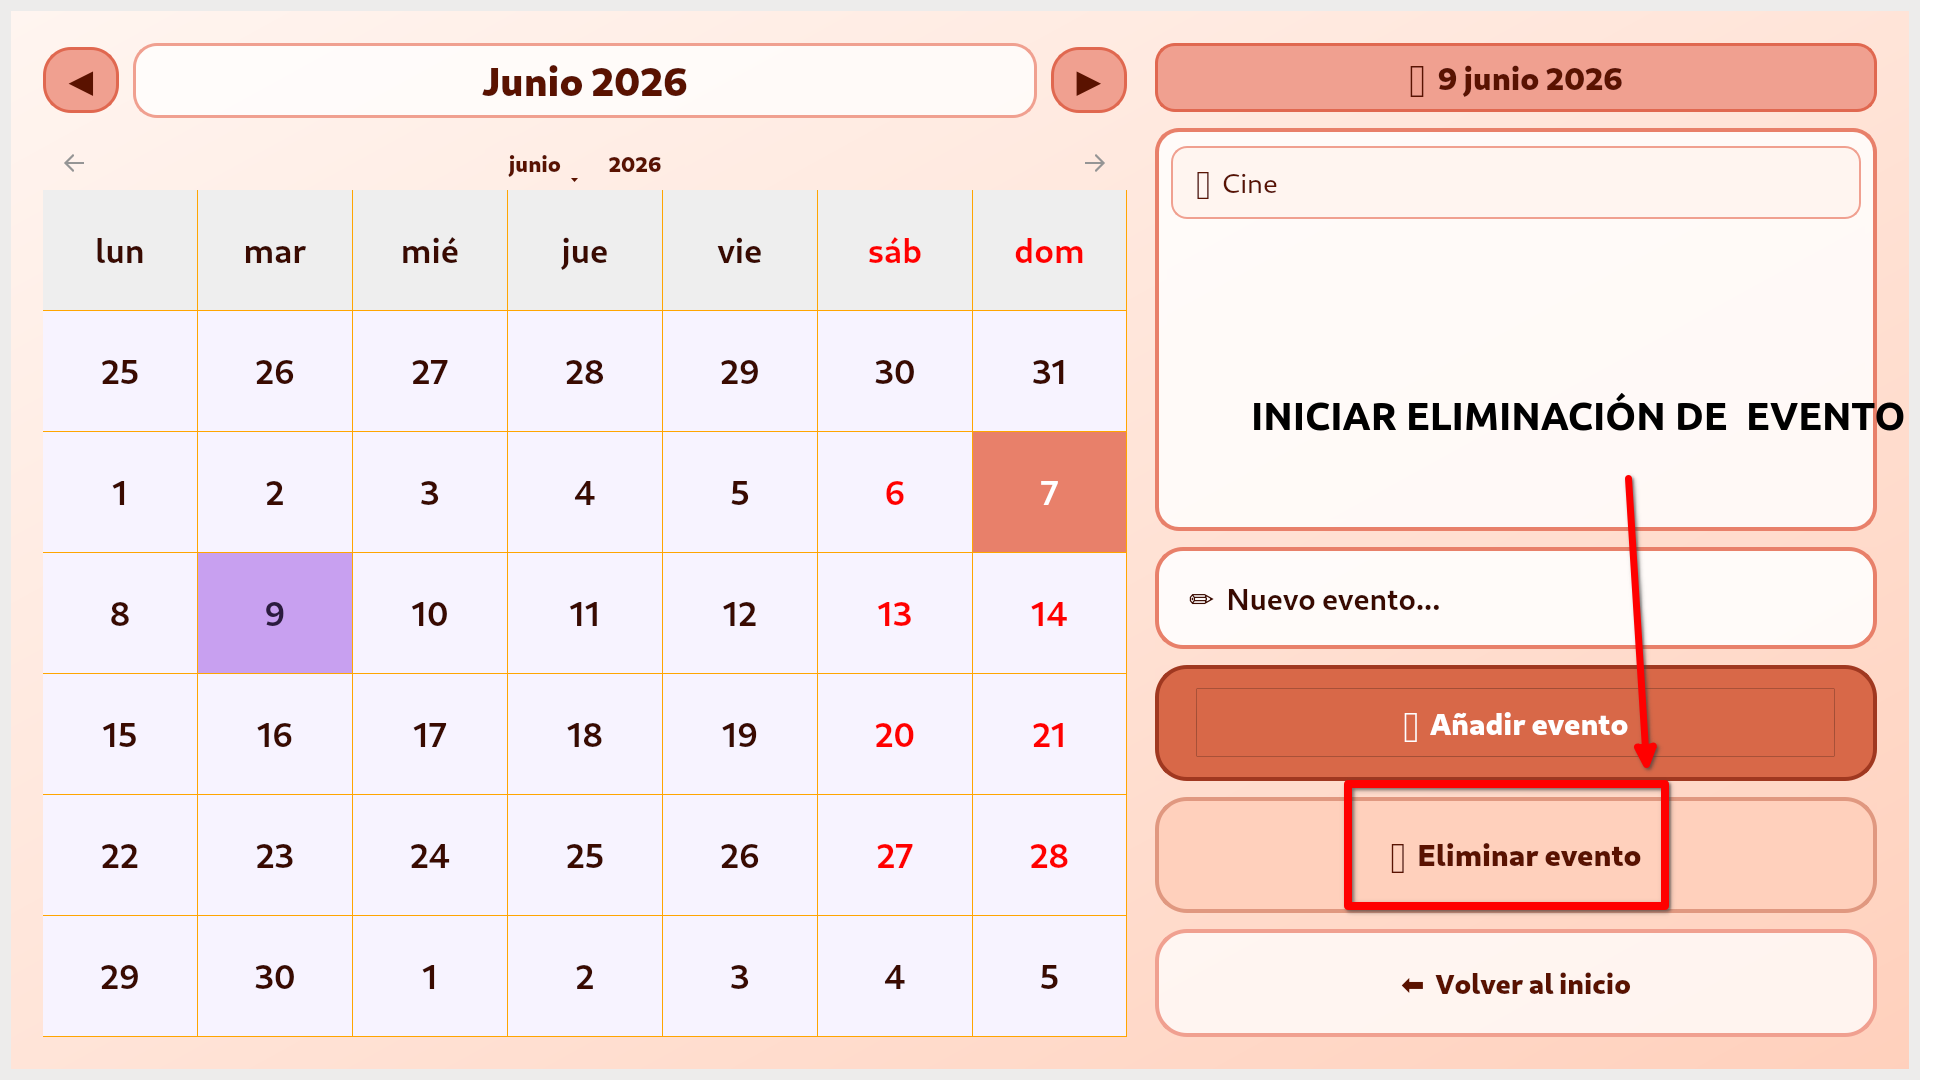
\includegraphics[width=0.9\textwidth]{figs/EL}
    \caption{Selección de evento a eliminar}
    \label{fig:EL}
\end{figure}


\begin{figure}[H]
    \centering
    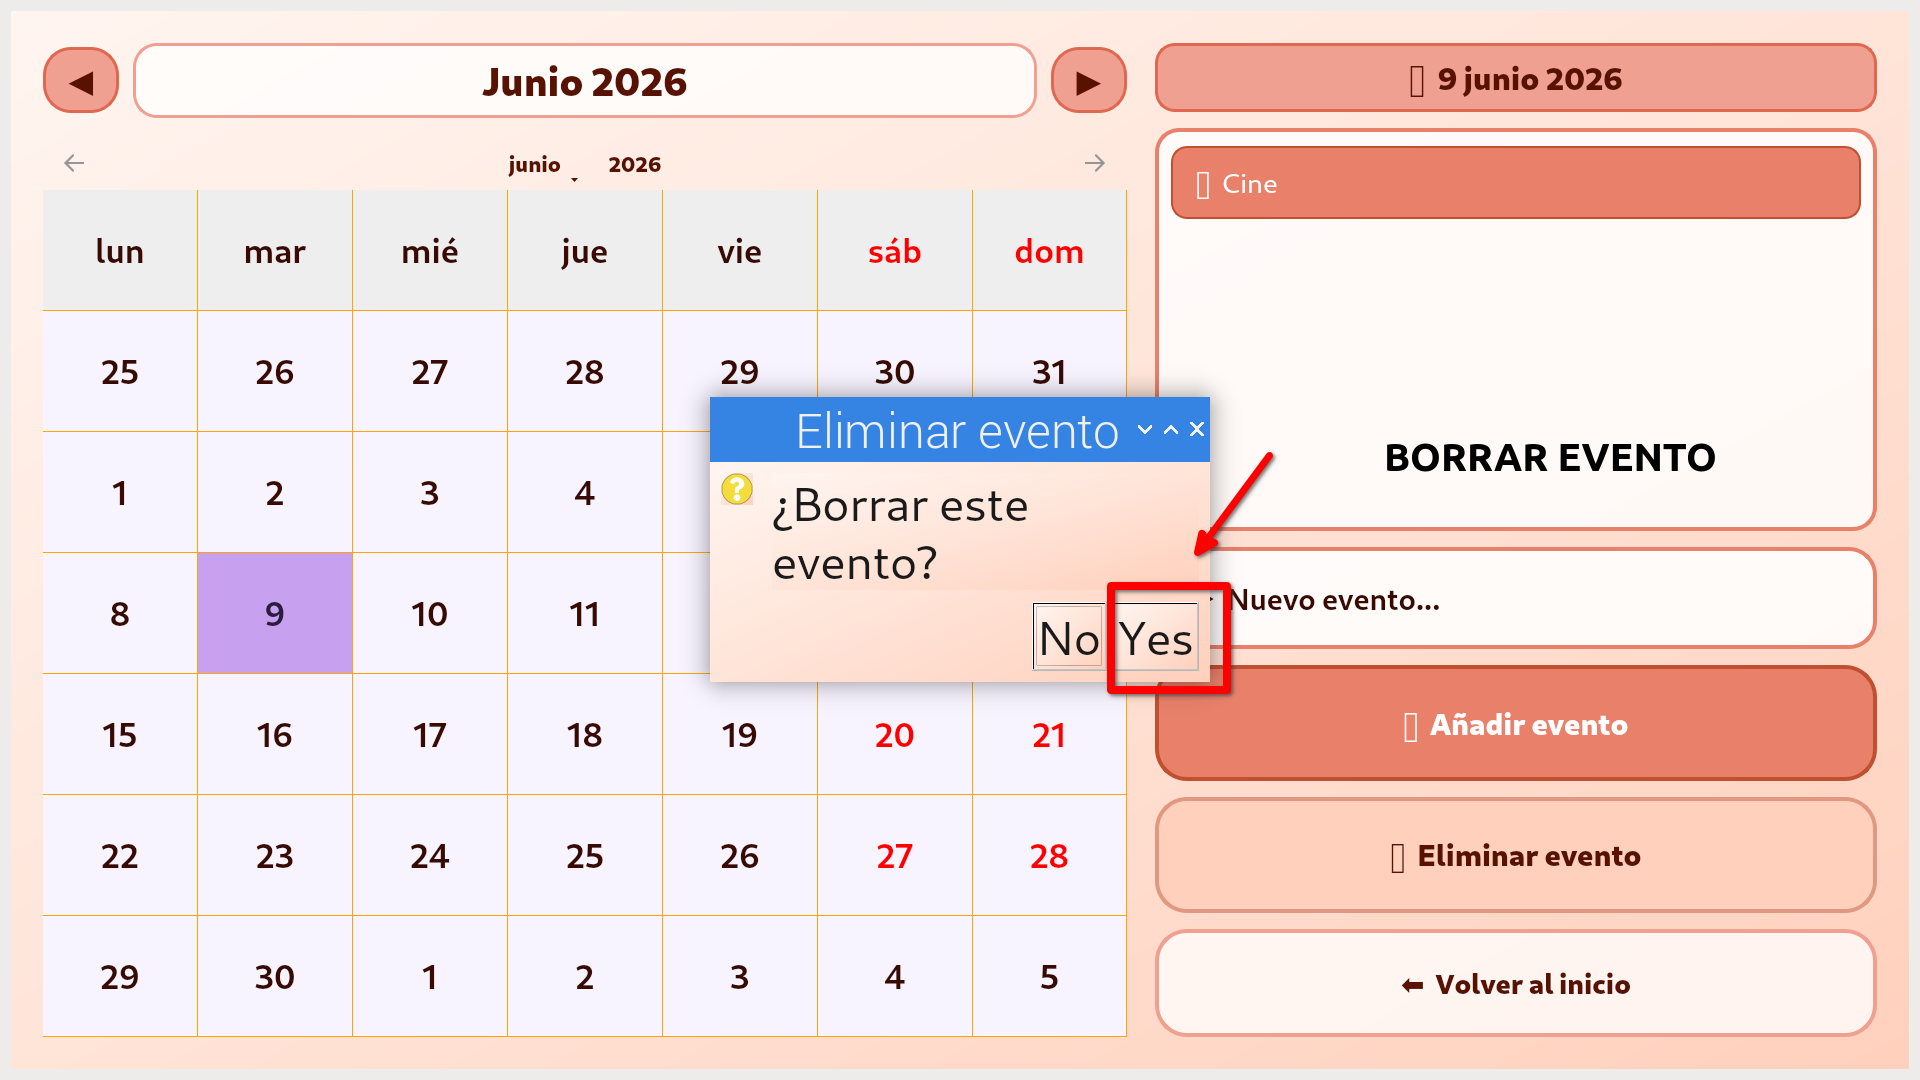
\includegraphics[width=0.9\textwidth]{figs/bo}
    \caption{Confirmación eliminación evento}
    \label{fig:bo}
\end{figure}



\subsection{Aplicación de recordatorios}

La aplicación de recordatorios permite programar avisos para una fecha y hora concretas.


\vspace{0.2cm}

\begin{figure}[H]
    \centering
    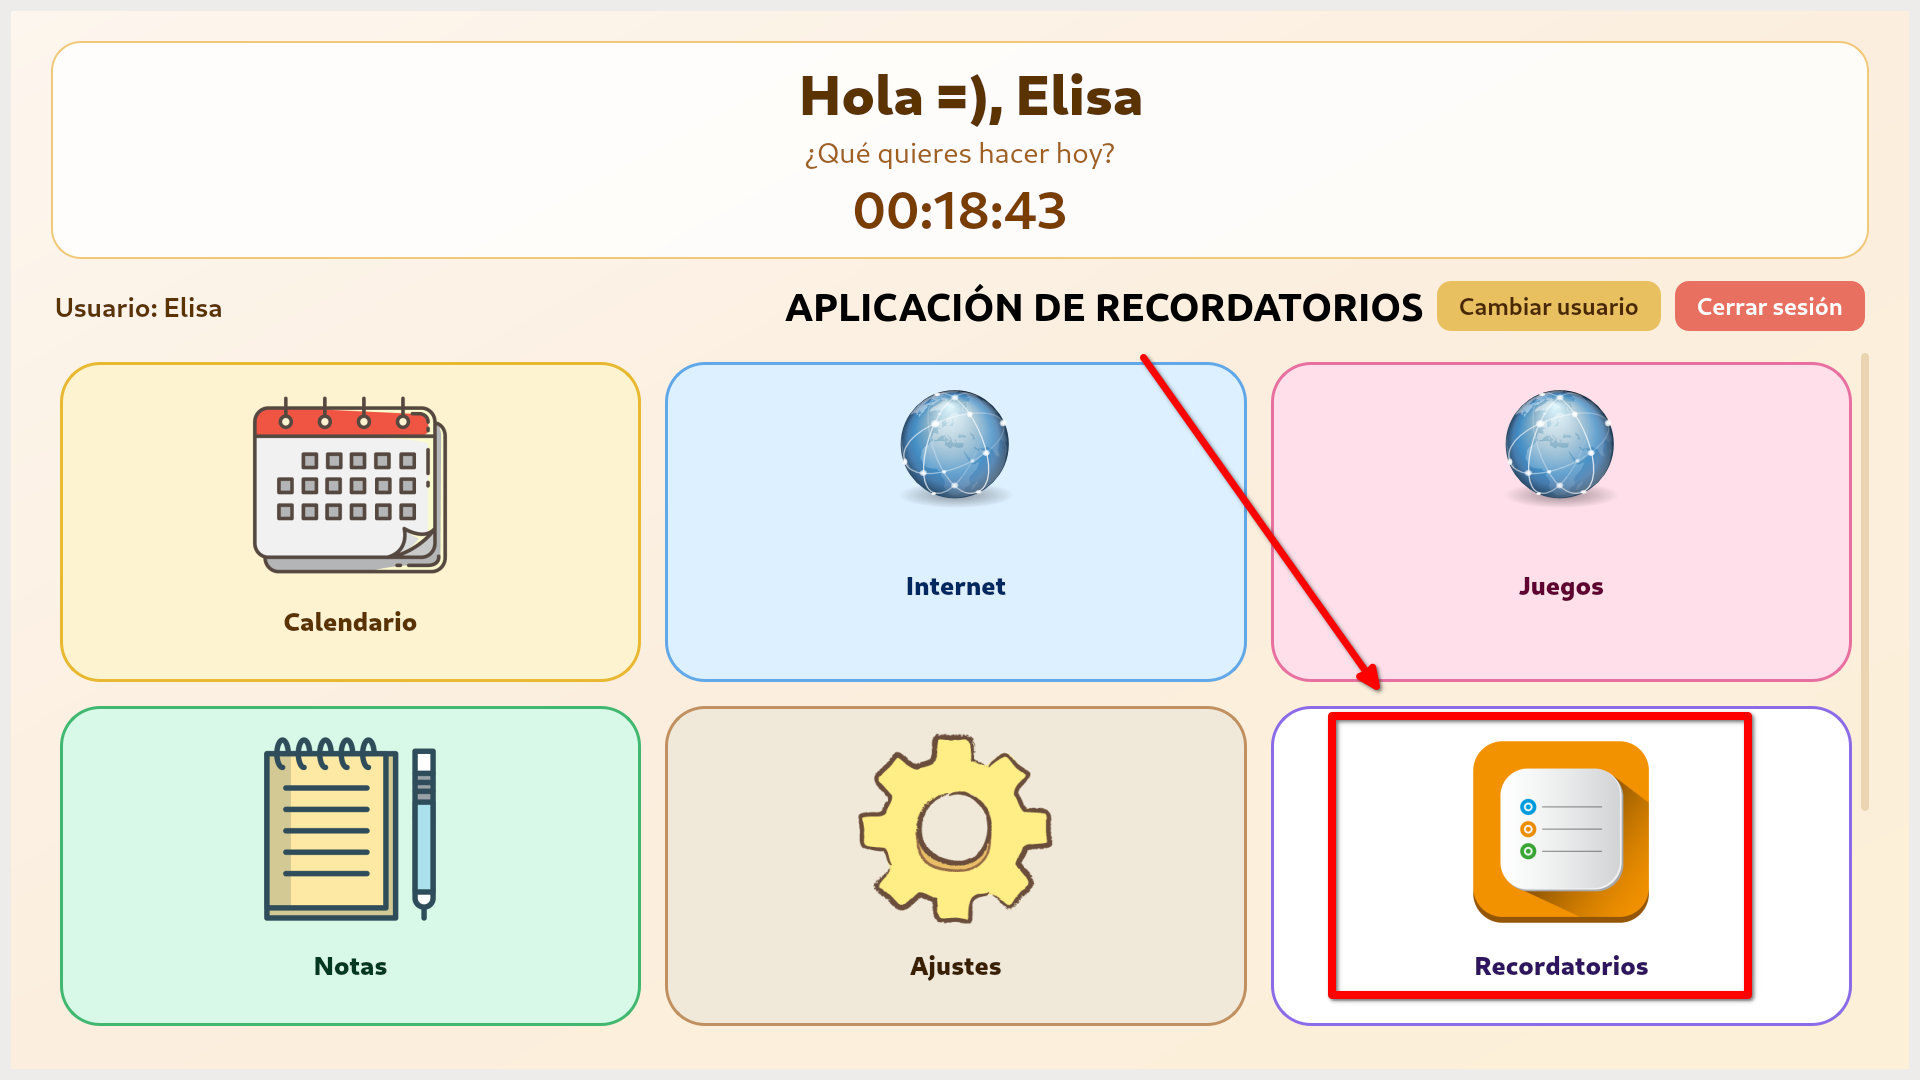
\includegraphics[width=0.9\textwidth]{figs/rec-app}
    \caption{Aplicación de recordatorios}
    \label{fig:rec-app}
\end{figure}



Para crear un nuevo recordatorio, se deben seguir los siguientes pasos:


\textbf{Paso 1:} Seleccionar fecha y hora del recordatorio.\\

El usuario selecciona la fecha y hora que desea añadir el recordatorio.


\begin{figure}[H]
    \centering
    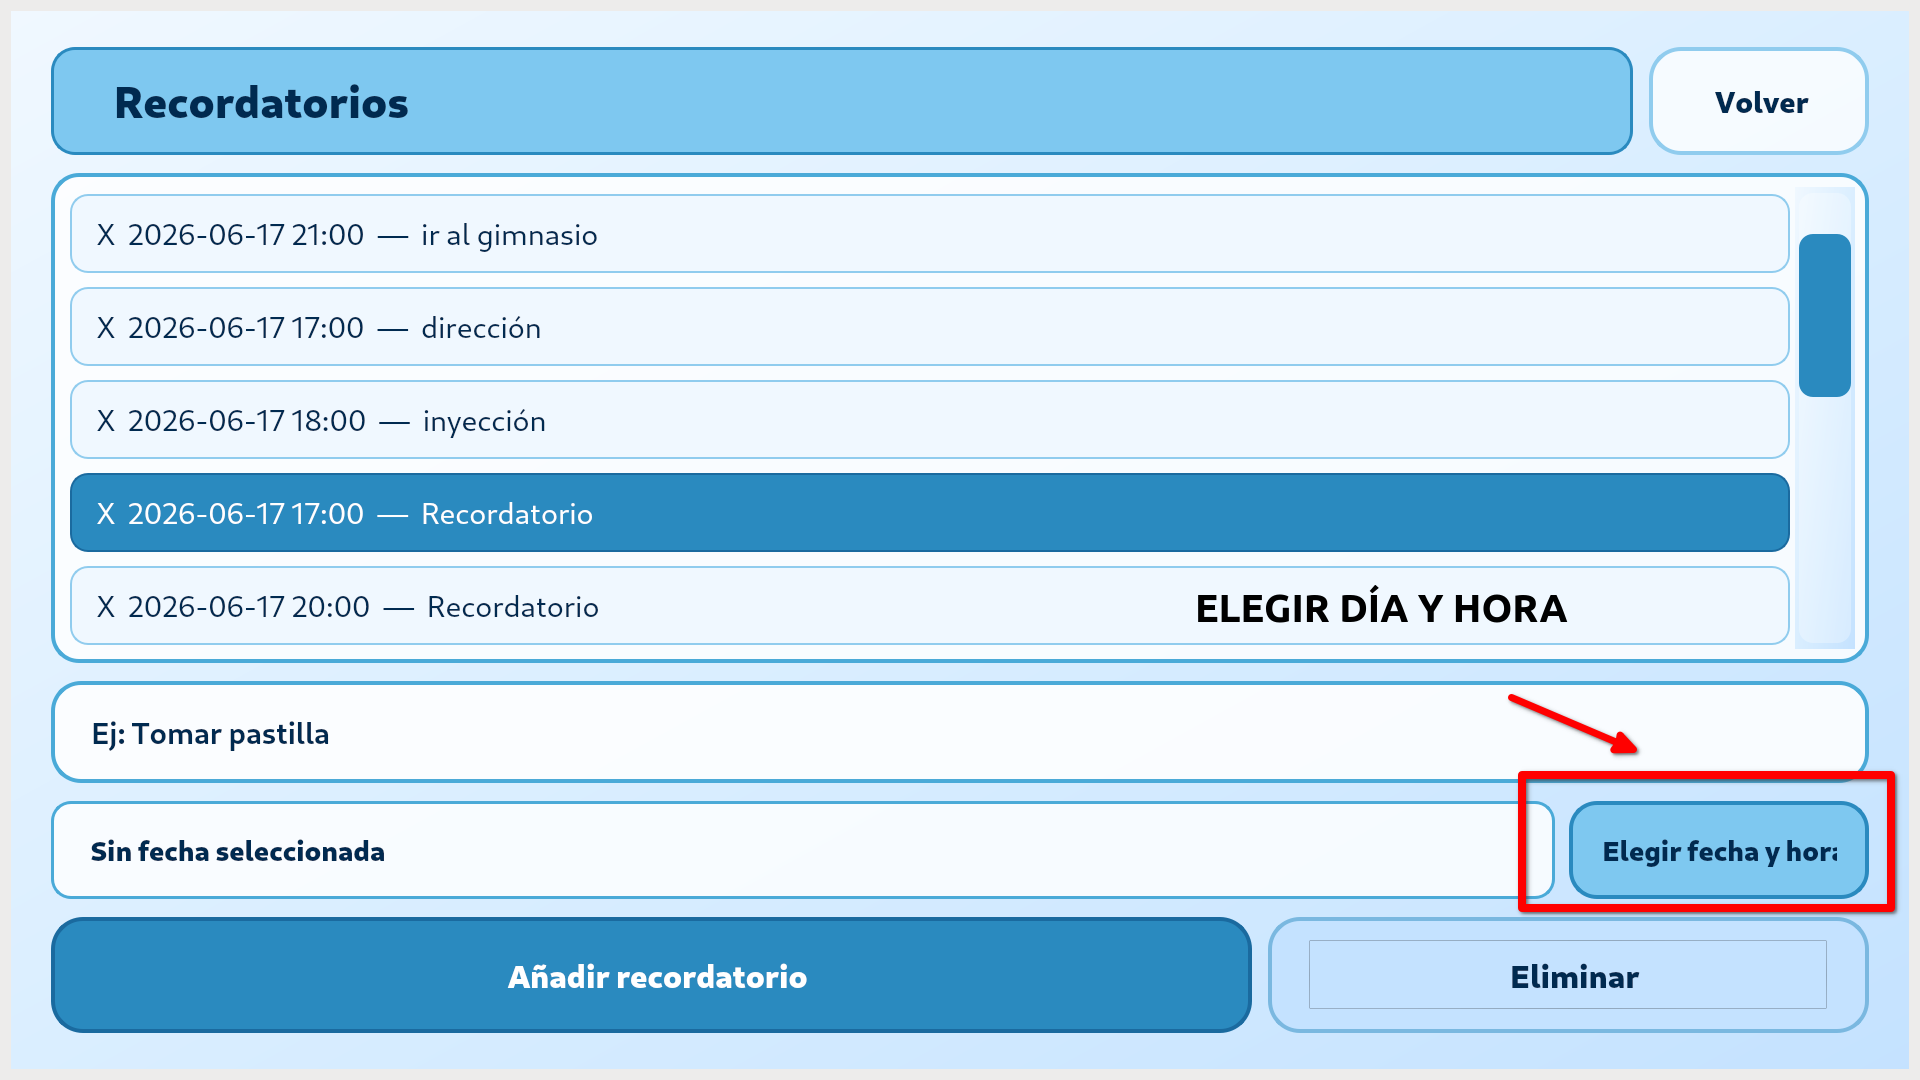
\includegraphics[width=0.9\textwidth]{figs/fecha}
    \caption{Elegir fecha recordatorio}
    \label{fig:fecha}
\end{figure}


\begin{figure}[H]
    \centering
    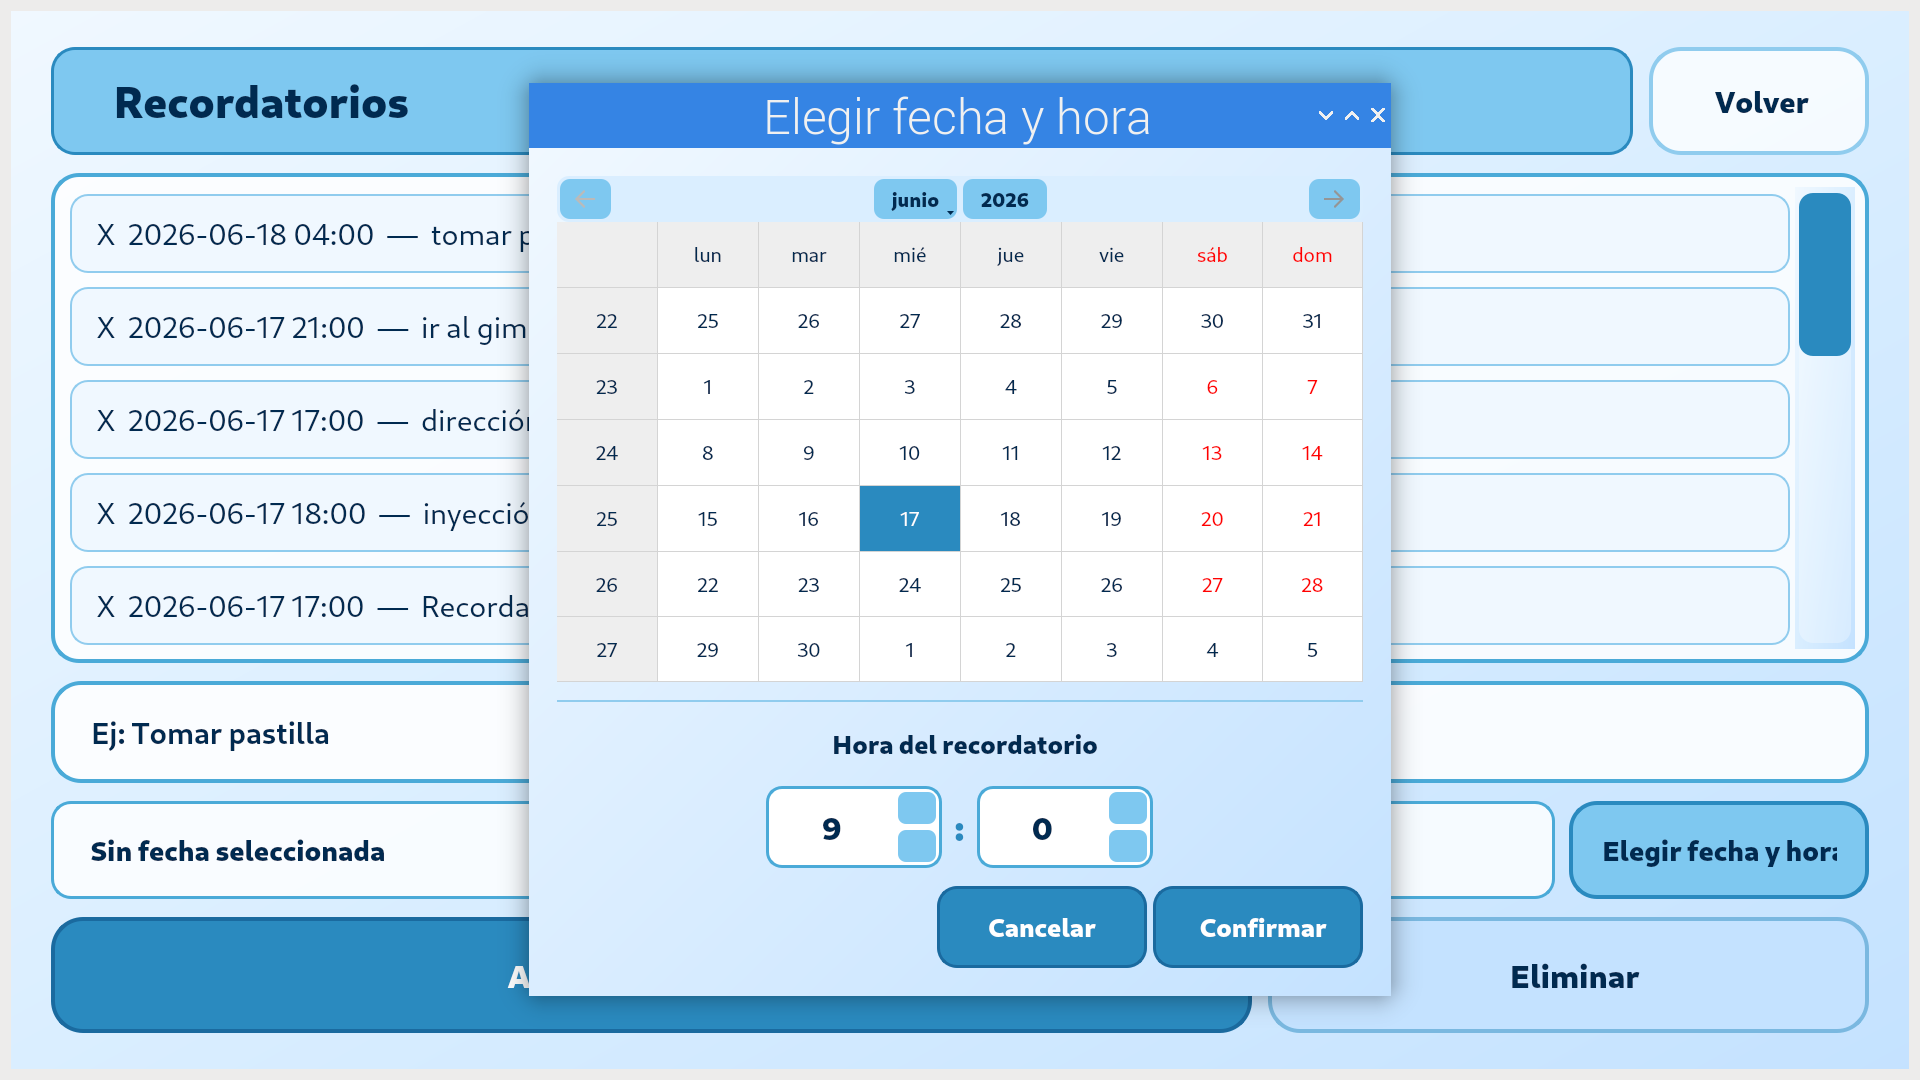
\includegraphics[width=0.9\textwidth]{figs/dia-rec}
    \caption{Calendario selector}
    \label{fig:dia-rec}
\end{figure}


\textbf{Paso 2:} Introducir el nombre del recordatorio.\\

Una vez seleccionada la fecha, se escribe el nombre del nuevo recordatorio.

\vspace{0.2cm}

\begin{figure}[H]
    \centering
    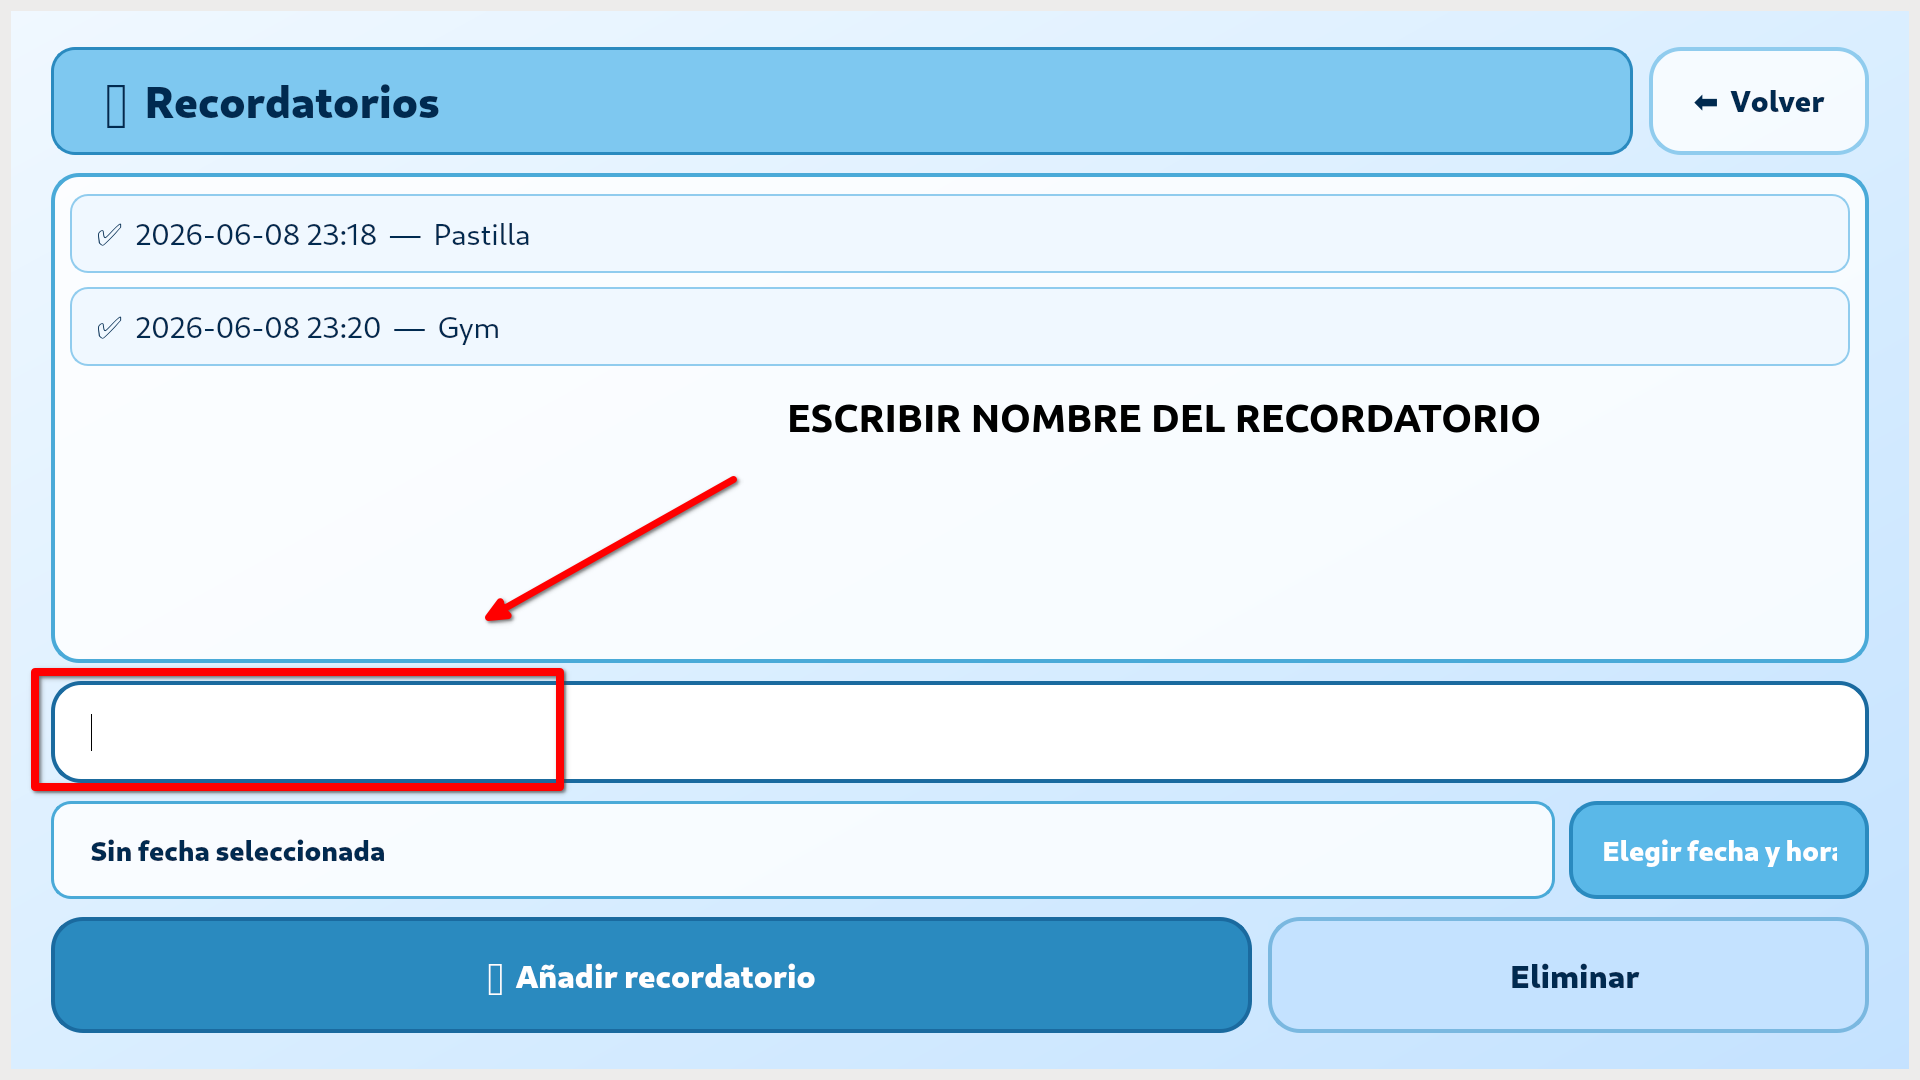
\includegraphics[width=0.9\textwidth]{figs/nombre-rec}
    \caption{Añadir nombre del recordatorio}
    \label{fig:nombre-rec}
\end{figure}


Tras crear el nuevo recordatorio, este se almacena en el sistema y se activará automáticamente en la fecha y hora programadas.

\vspace{0.2cm}


\subsection{Aplicación de notas}

La aplicación de notas permite añadir, consultar, buscar y eliminar notas de forma sencilla.

\vspace{0.2cm}

\begin{figure}[H]
    \centering
    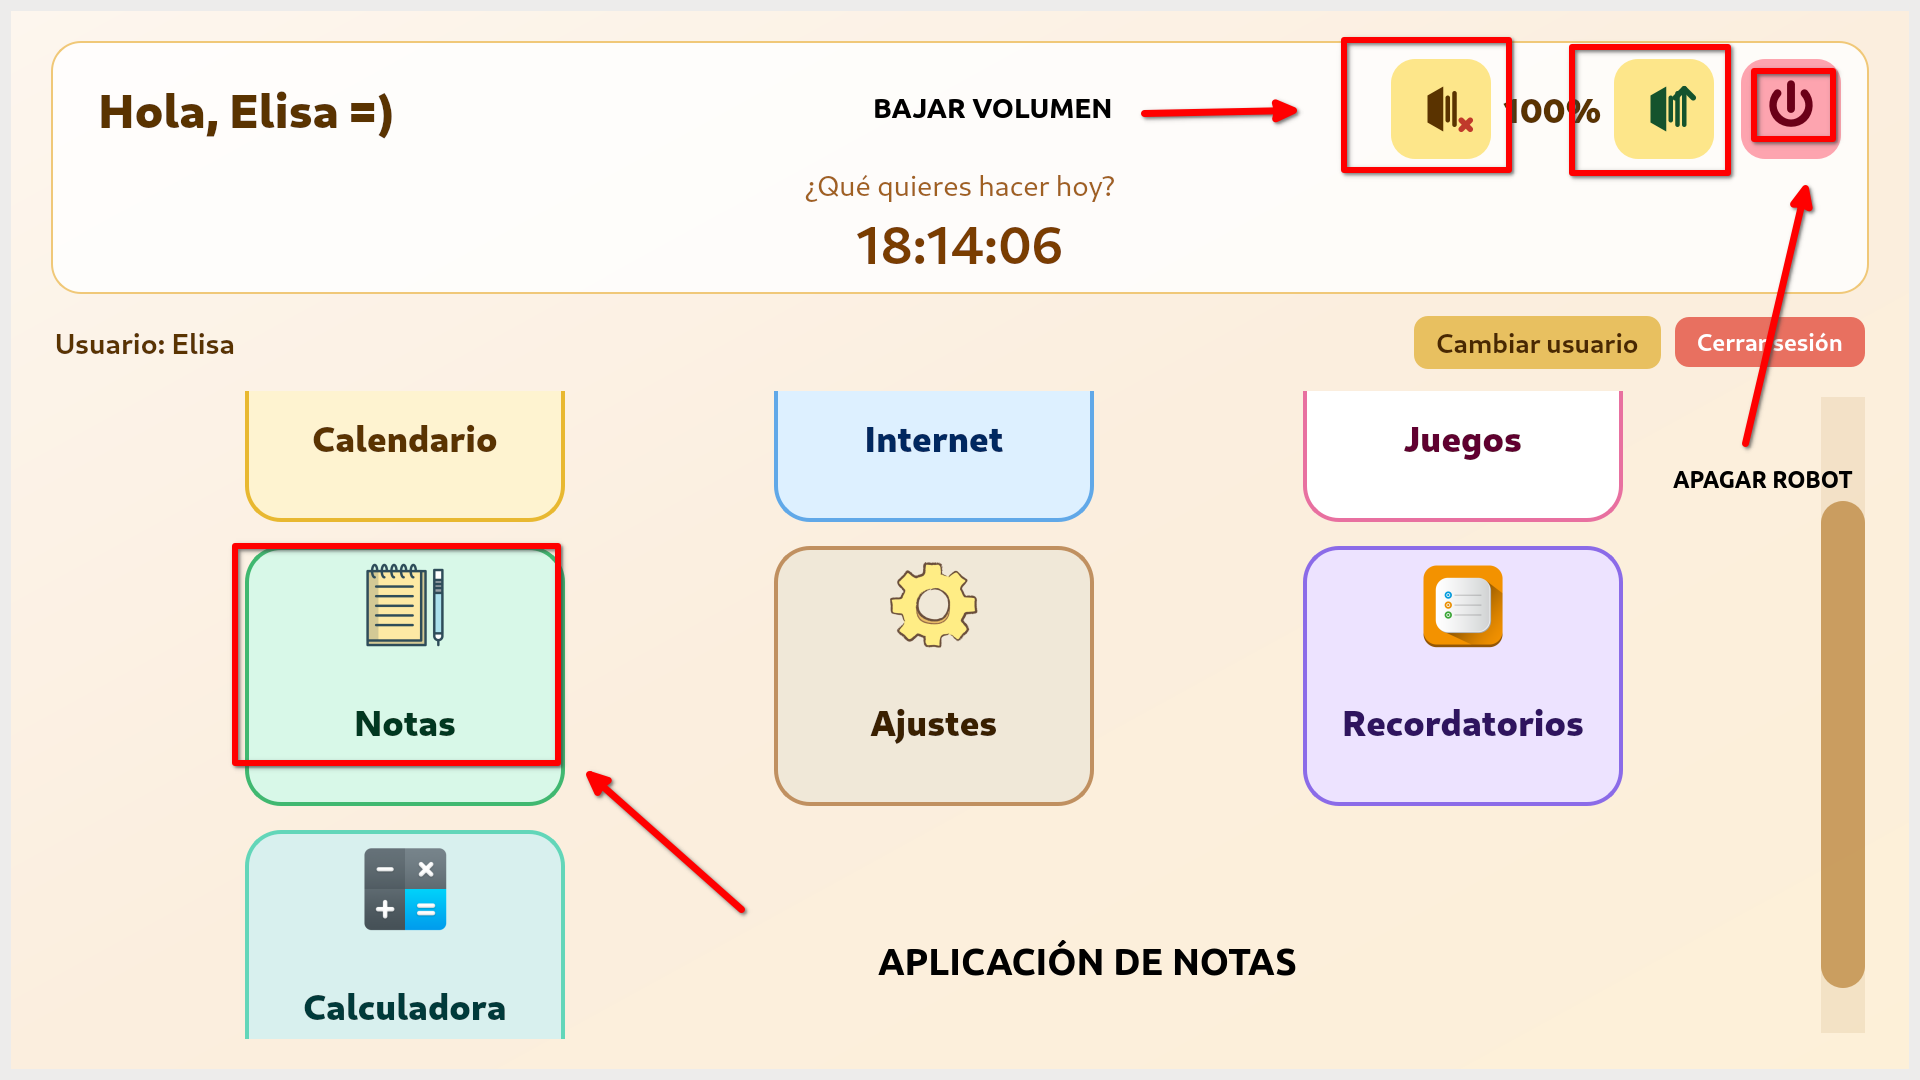
\includegraphics[width=0.9\textwidth]{figs/not}
    \caption{Aplicación de notas}
    \label{fig:not}
\end{figure}


Para crear una nueva nota, el usuario debe introducir un título y el contenido correspondiente.

\vspace{0.2cm}

\begin{figure}[H]
    \centering
    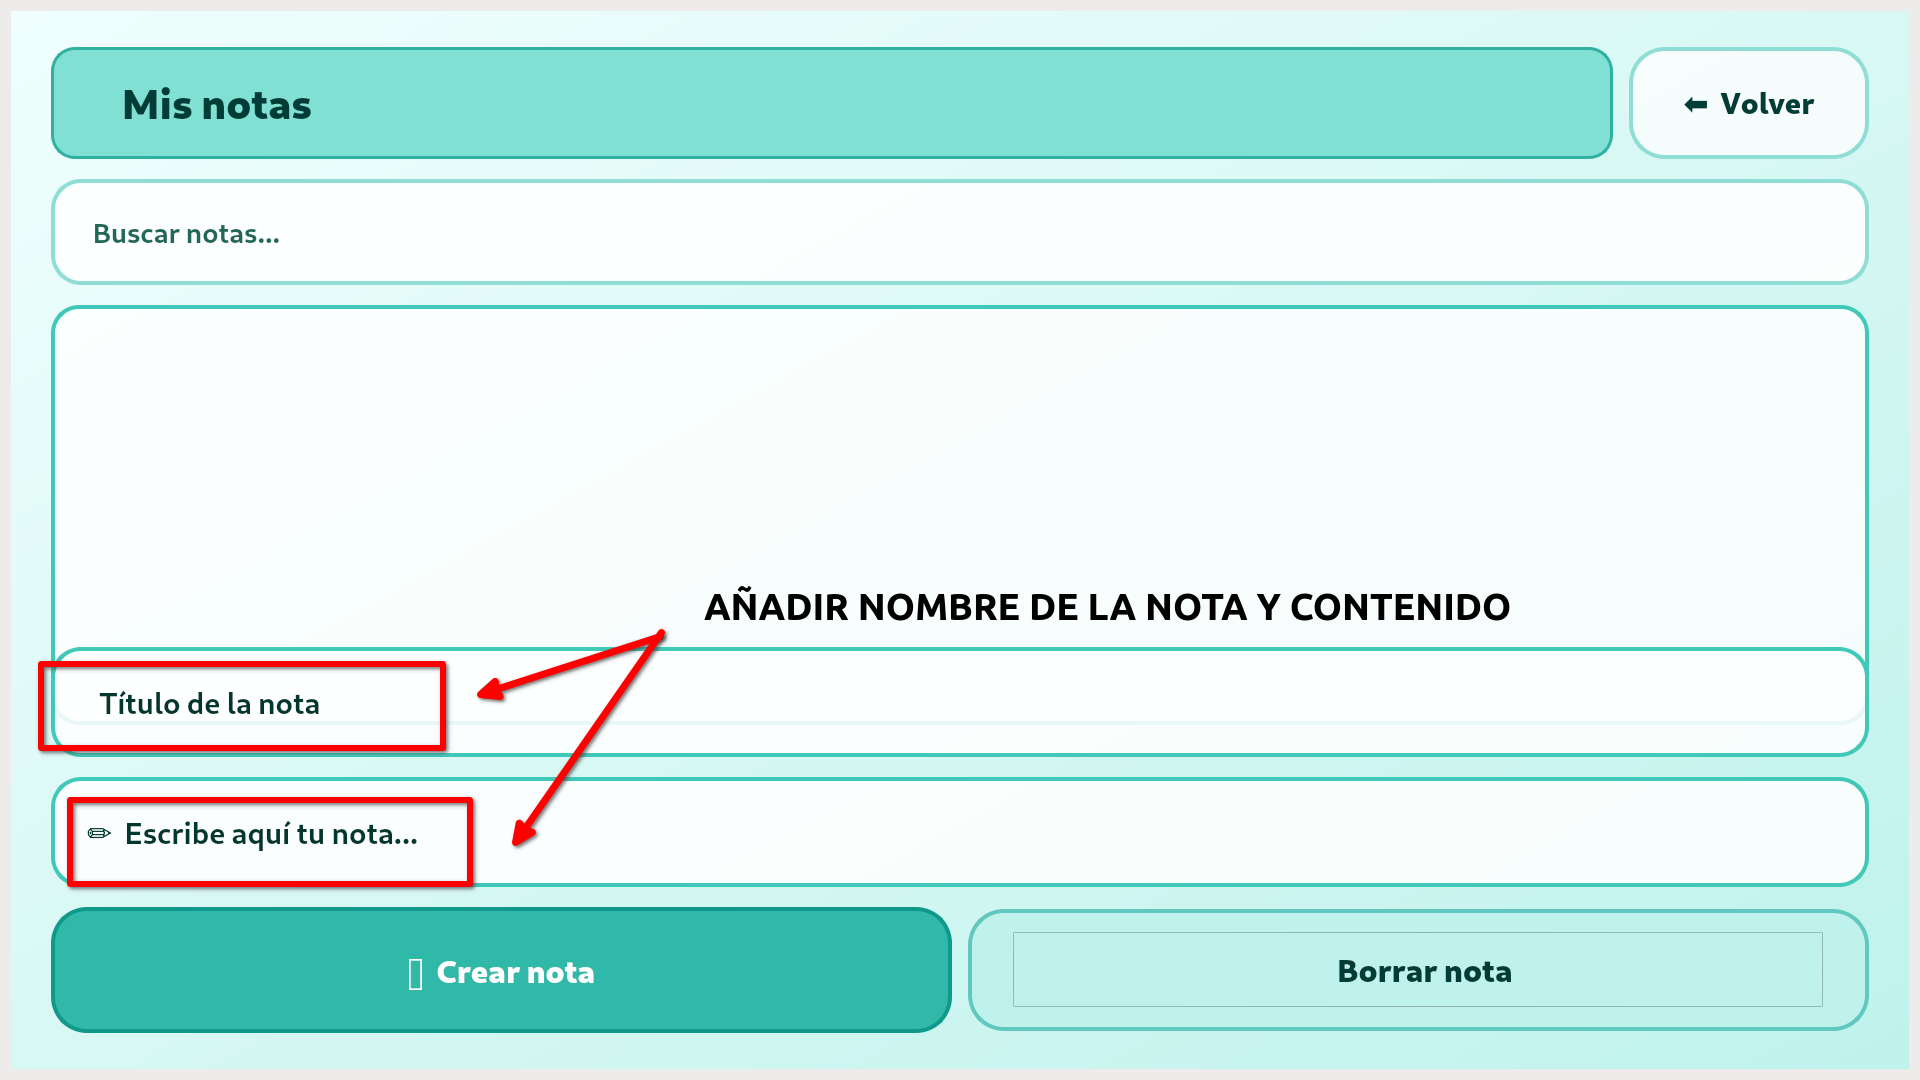
\includegraphics[width=0.9\textwidth]{figs/notas-add}
    \caption{Añadir contenido de la nota}
    \label{fig:notas-add}
\end{figure}

\vspace{0.2cm}


\begin{figure}[H]
    \centering
    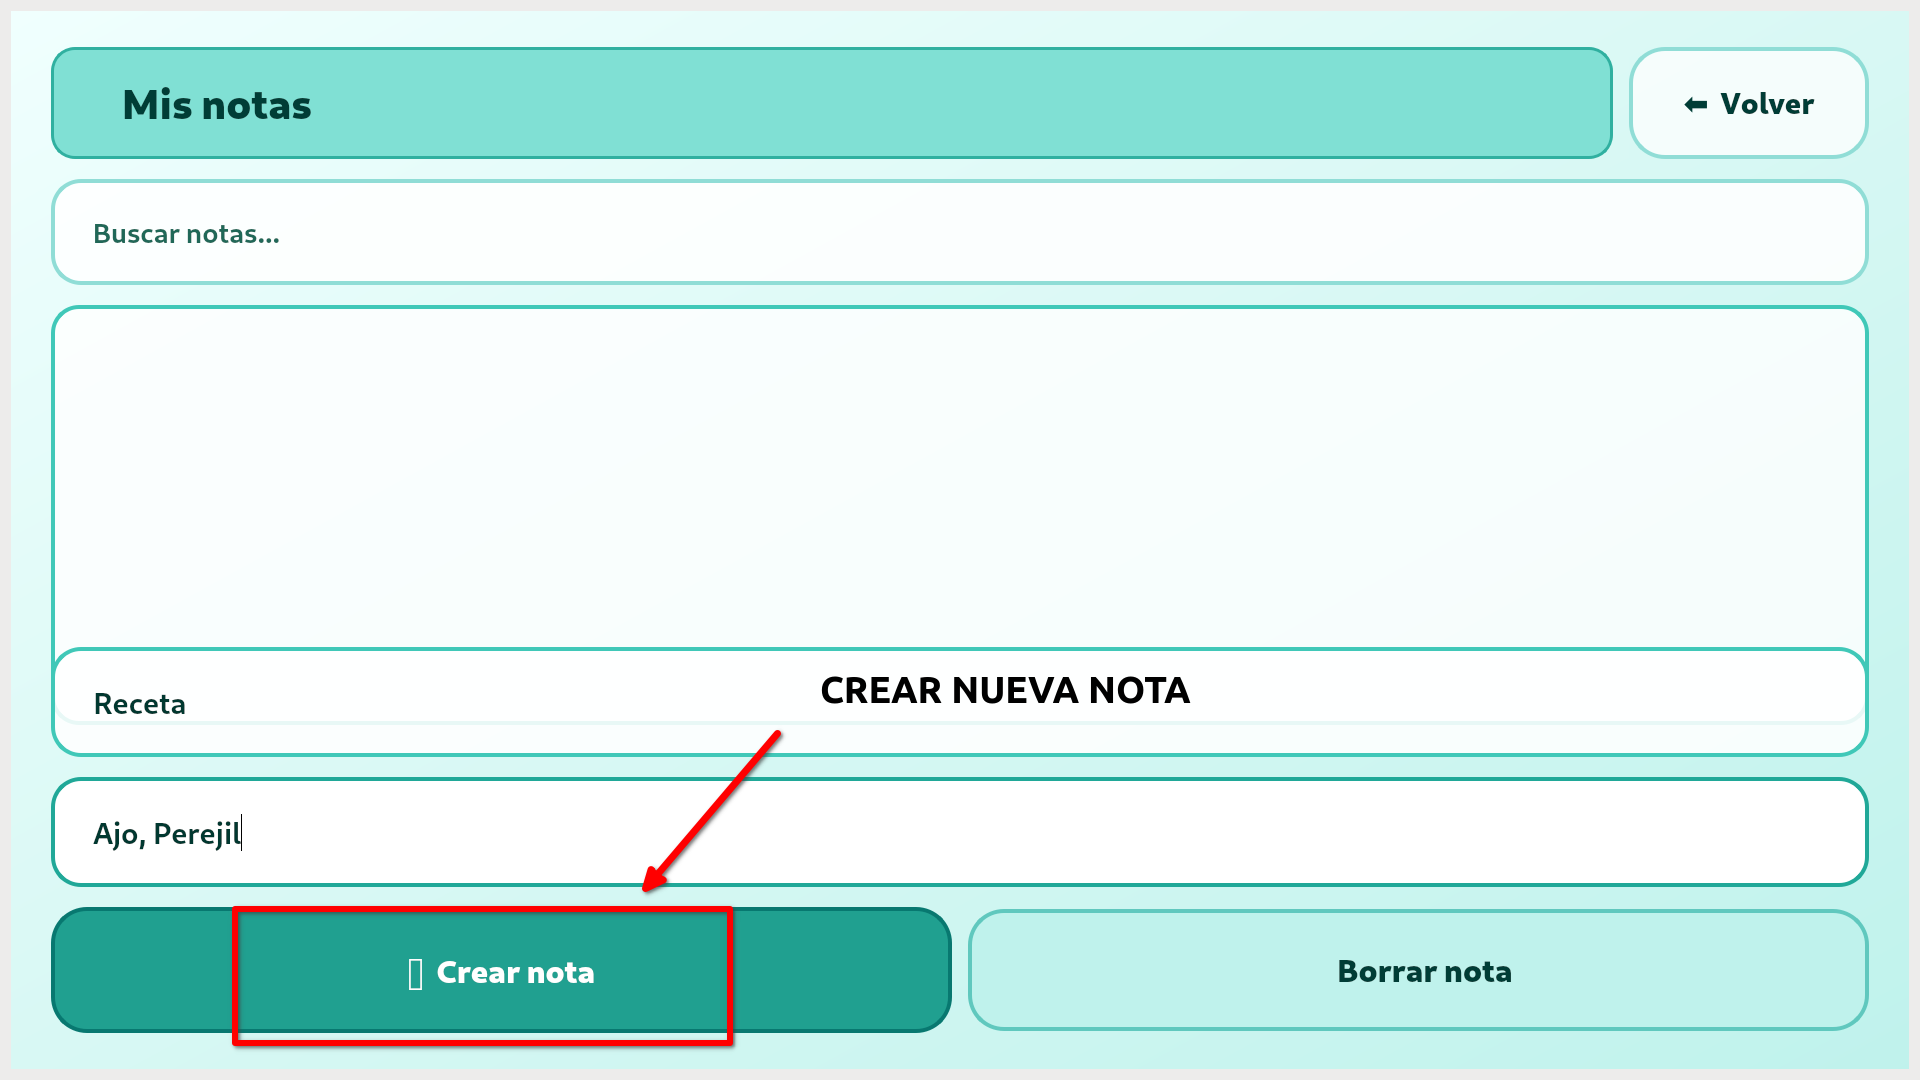
\includegraphics[width=0.9\textwidth]{figs/nota-add2}
    \caption{Crear la nueva nota}
    \label{fig:nota-add2}
\end{figure}


\vspace{0.2cm}

\begin{figure}[H]
    \centering
    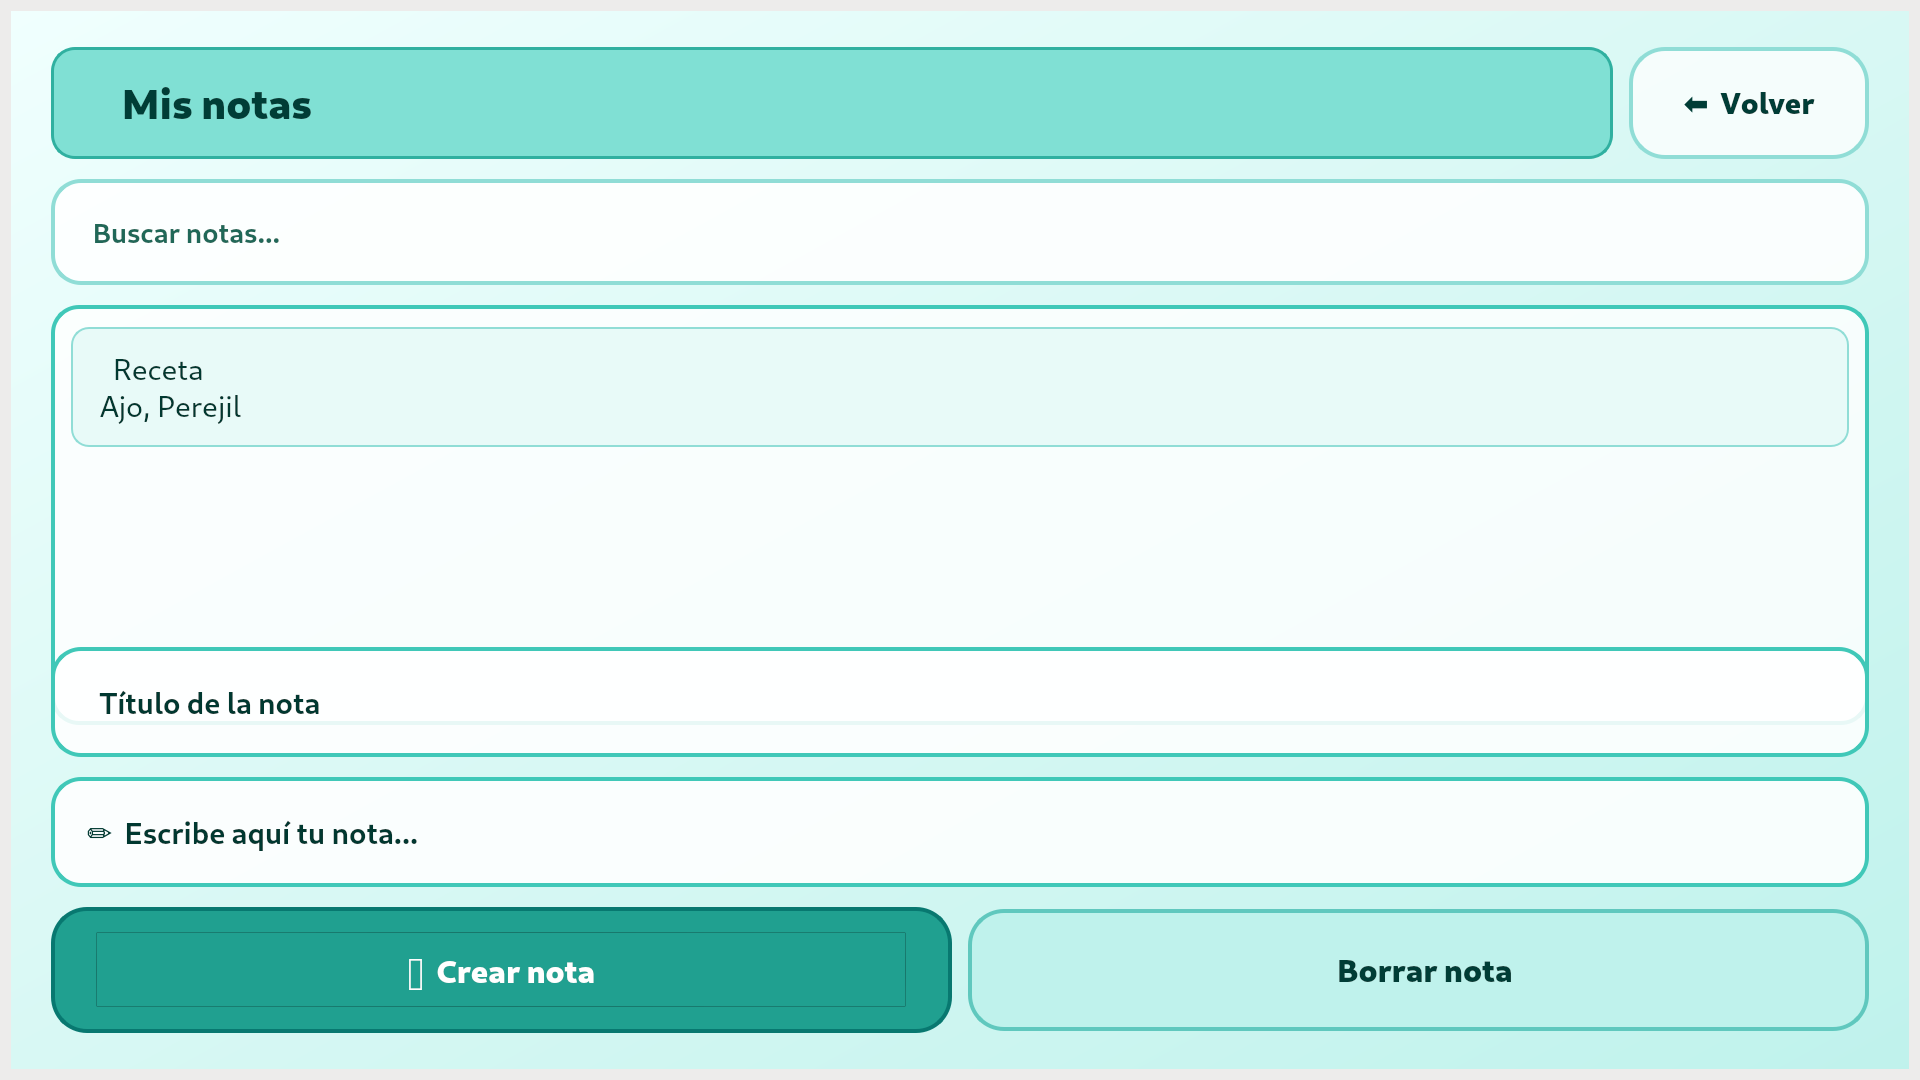
\includegraphics[width=0.9\textwidth]{figs/not-cre}
    \caption{Nota creada}
    \label{fig:not-cre}
\end{figure}

Además de crear y eliminar una nueva nota, la aplicación permite buscar notas a partir de su título.

\vspace{0.2cm}

\begin{figure}[H]
    \centering
    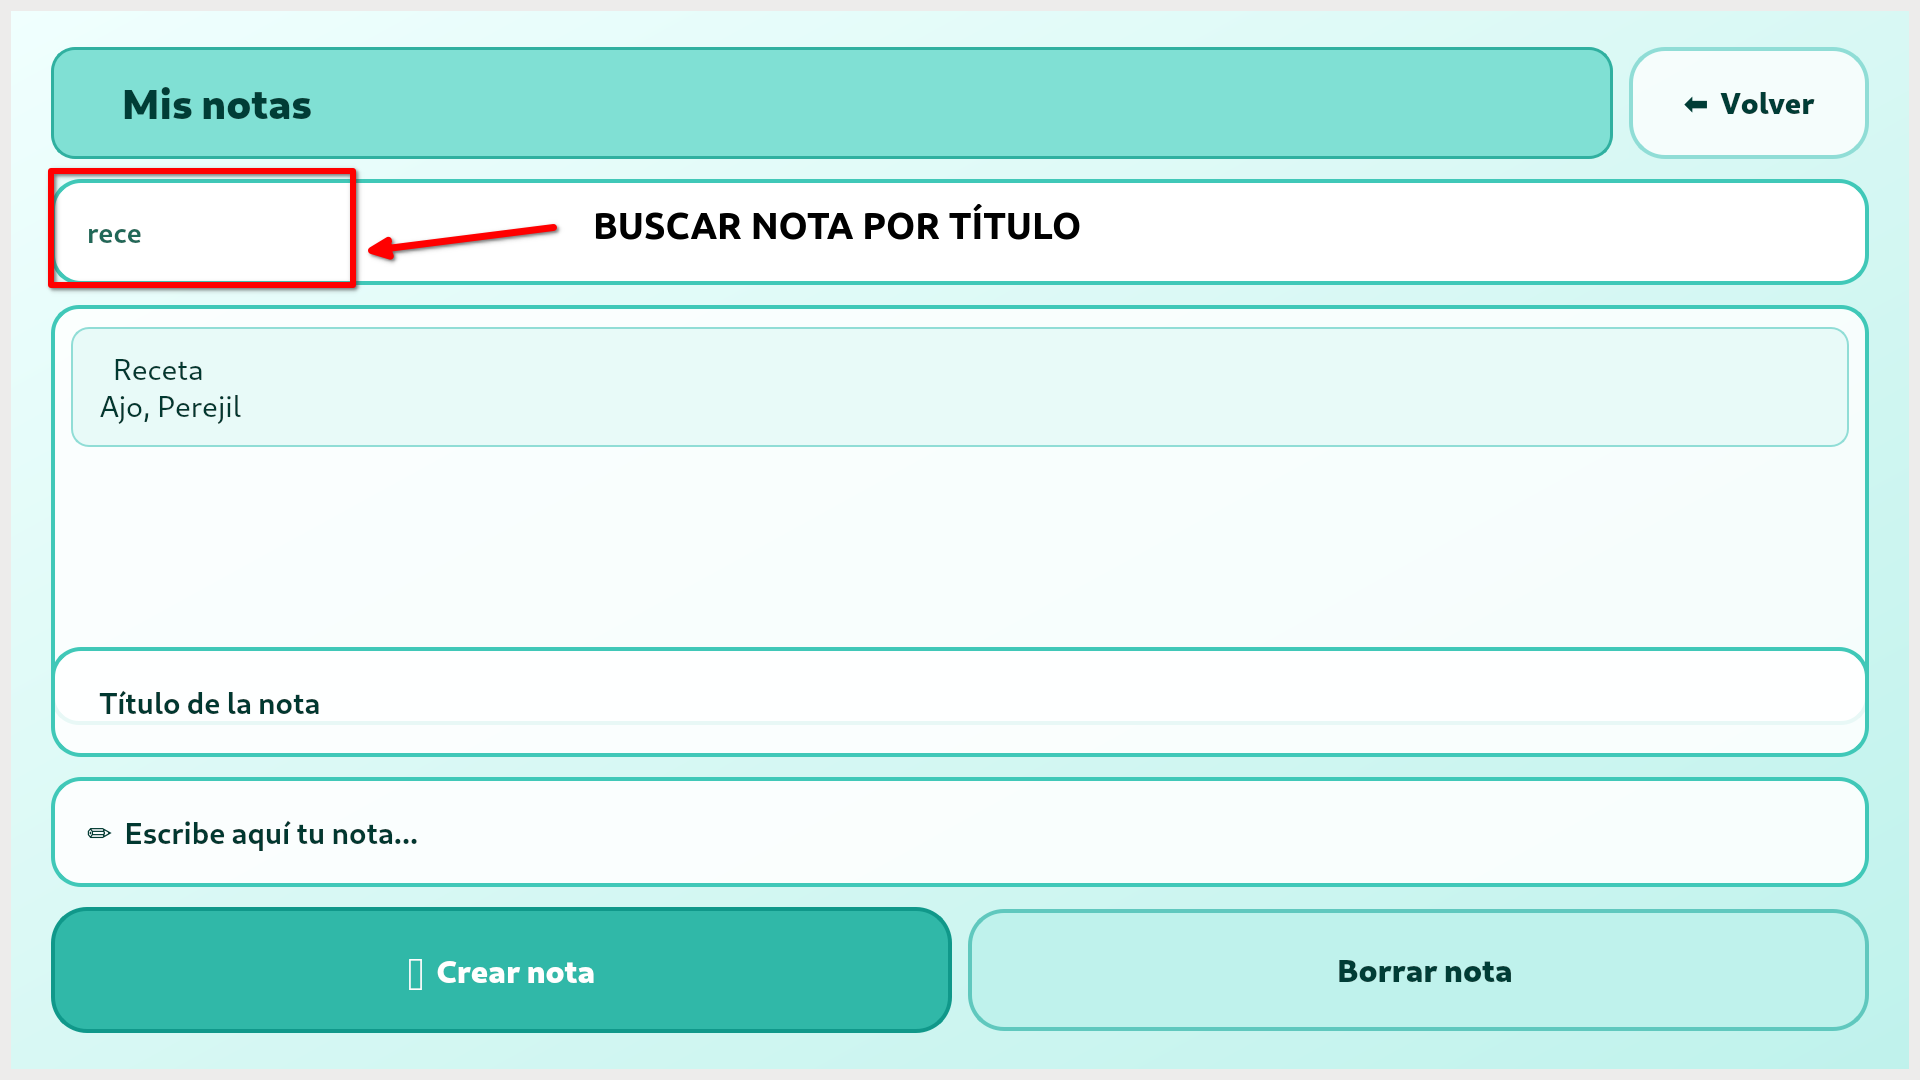
\includegraphics[width=0.9\textwidth]{figs/buscar}
    \caption{Buscar nota}
    \label{fig:buscar}
\end{figure}


\subsection{Aplicación de navegador web}

La aplicación de navegador web permite acceder a Internet y realizar búsquedas sin abandonar la interfaz del robot.

\vspace{0.2cm}

\begin{figure}[H]
    \centering
    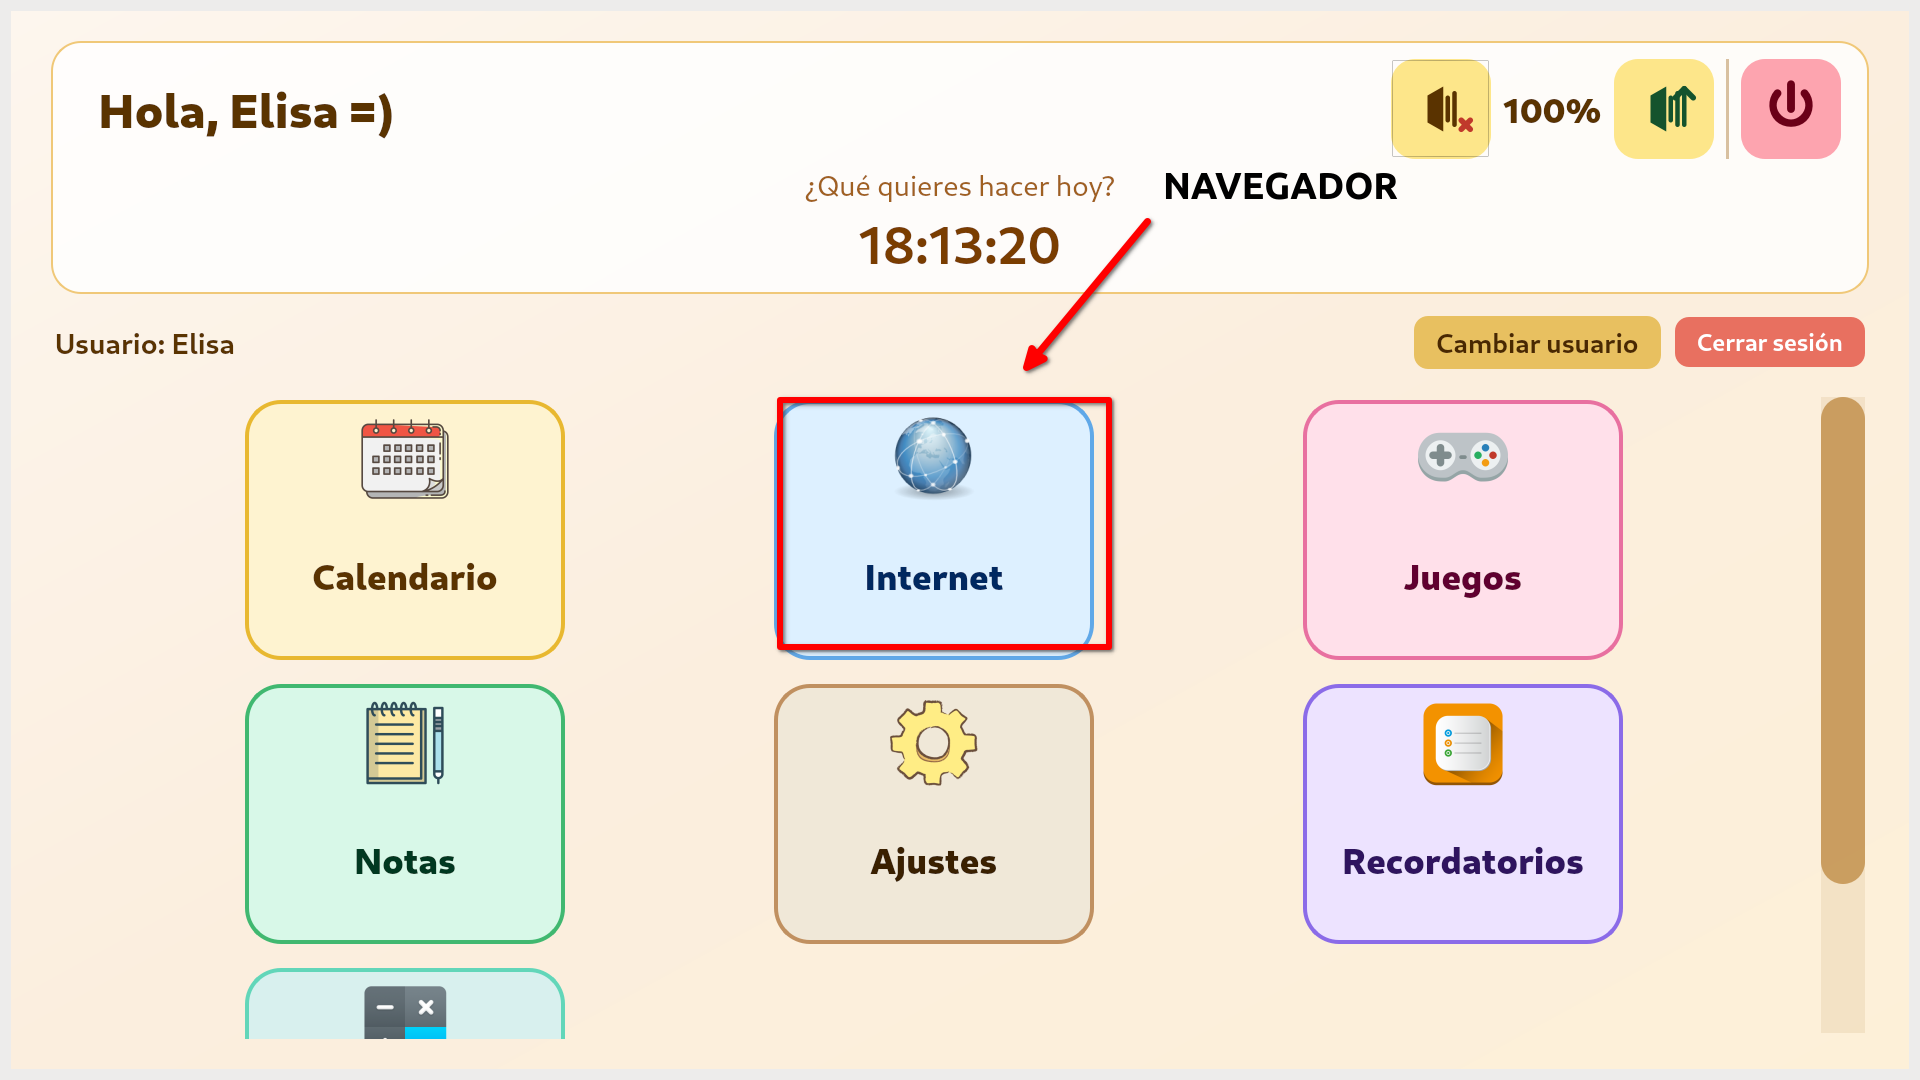
\includegraphics[width=0.9\textwidth]{figs/web-app}
    \caption{Aplicación navegador web página principal}
    \label{fig:web-app}
\end{figure}


\vspace{0.2cm}

\begin{figure}[H]
    \centering
    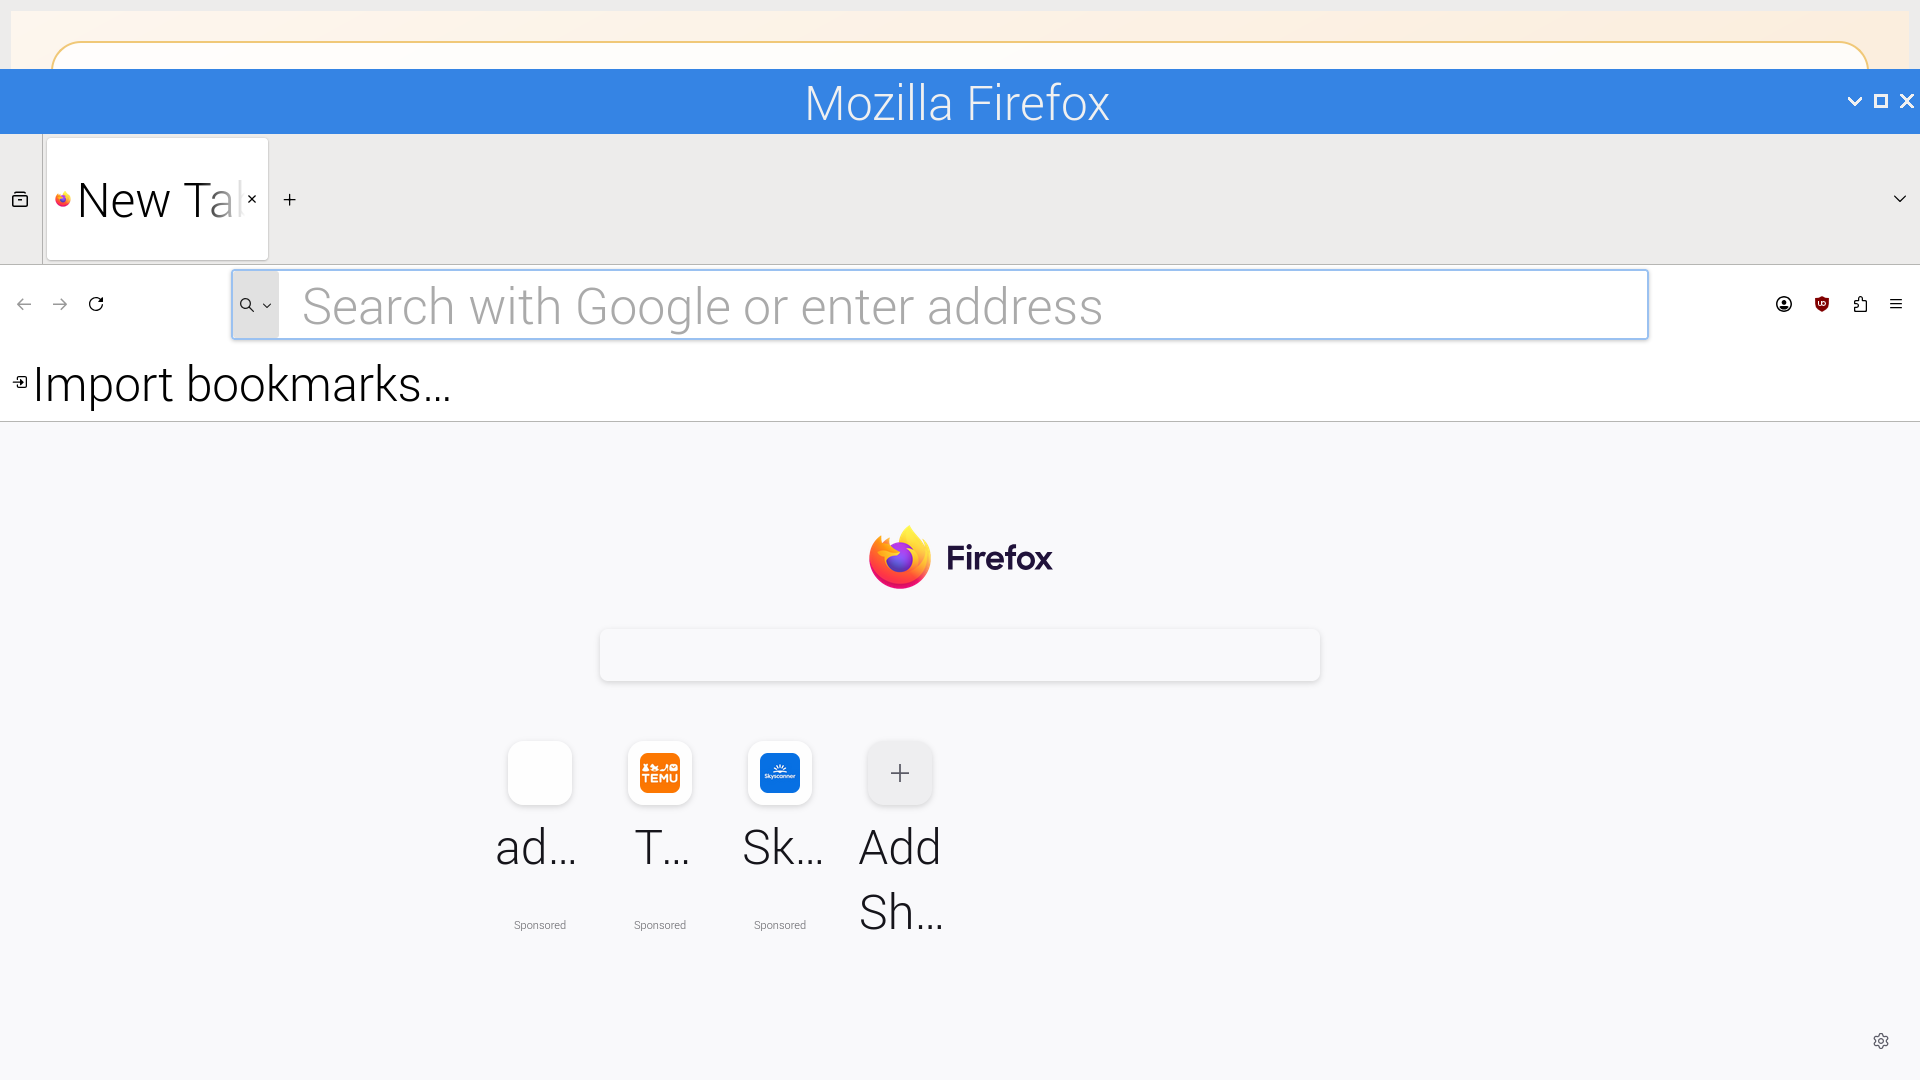
\includegraphics[width=0.9\textwidth]{figs/web}
    \caption{Aplicación navegador web}
    \label{fig:web}
\end{figure}



Además de las aplicaciones descritas, la pantalla principal incorpora controles rápidos para poder ajustar el volumen del sistema y apagar el robot de forma segura.

\vspace{0.2cm}

\begin{figure}[H]
    \centering
    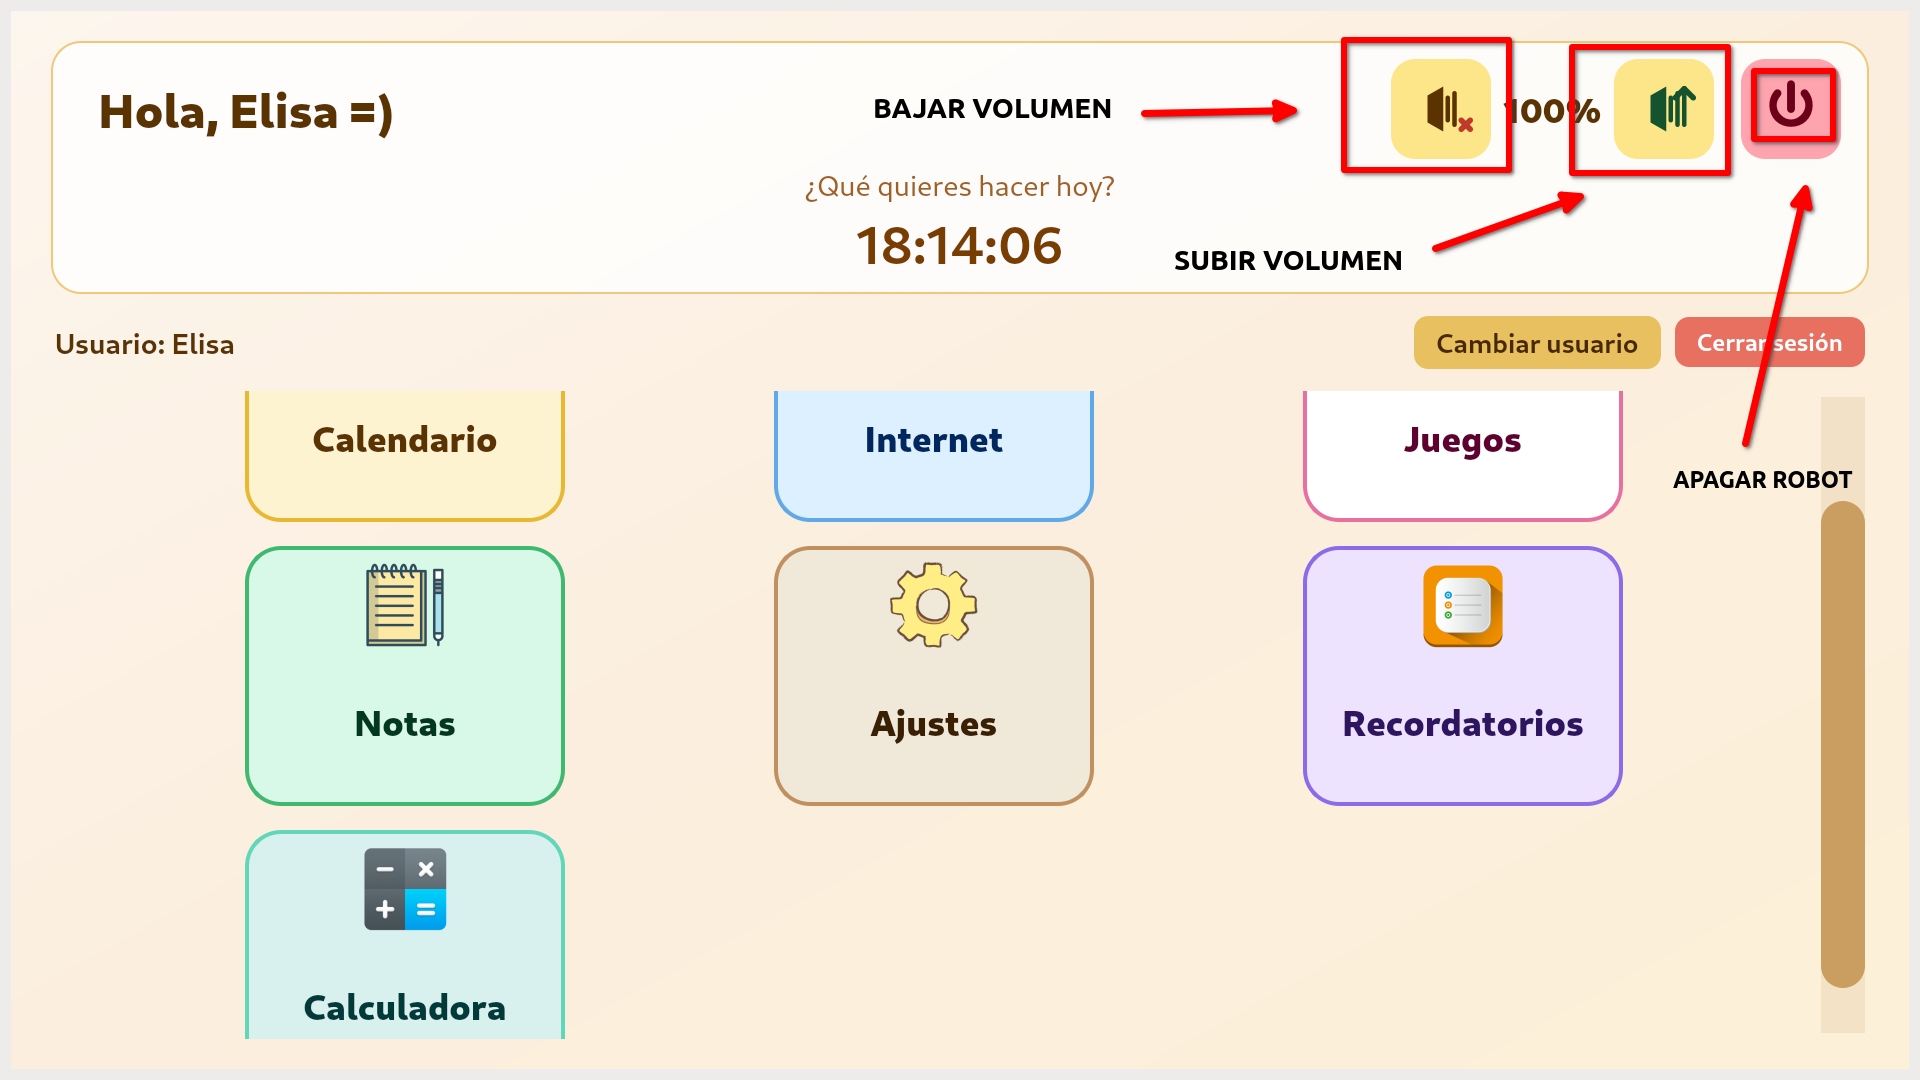
\includegraphics[width=0.9\textwidth]{figs/vol}
    \caption{Controles de volumen y apagado del sistema}
    \label{fig:vol}
\end{figure}


\section{Problemas frecuentes}

Durante el uso del sistema pueden producirse las siguientes incidencias habituales:

\begin{itemize}
	\item La cámara no detecta al usuario en condiciones de iluminación insuficiente.
    \item El reconocimiento de voz puede interpretar incorrectamente una orden debido a una pronunciación poco clara o al ruido ambiente.
    \item El robot no detecta las palabras de parada.
\end{itemize}


En conjunto, la interfaz y las funcionalidades implementadas facilitan una interacción sencilla e intuitiva con el robot.

